\documentclass[
    12pt, % font size
    parskip=half, % space between paragraphs instead of indentation
    print, % digital or print
    oneside, % oneside / twoside
    %	openright, % openright for title page and subsequent chapters on right pages in twosided layout
]{thesis}

\usepackage{microtype}

\usepackage{booktabs, enumitem, afterpage}

\usepackage{amssymb}
\usepackage{mathtools}
\usepackage{gensymb}
\usepackage{graphicx}
\usepackage{subfigure}
\usepackage{rotating}
\usepackage{acronym}

\usepackage{cleveref}
\usepackage{enumitem}

\usepackage{datetime}
\renewcommand{\dateseparator}{.}

\title{On the Impact of Submesoscale Fronts on Mesoscale Eddies and Biological Productivity in the California Current System}
\author{Max Simon}
\date{December 19, 2020}

\addbibresource{references.bib}

%% Hypothesis Design
\newcounter{hypothesis}
\newenvironment{hypothesis}%
{
    \begin{enumerate}[label=\textbf{H\arabic*:}, ref=H\arabic*, rightmargin=0.8cm, leftmargin=1.5cm, labelsep=0.6cm]
        \setcounter{enumi}{\thehypothesis}
        \item \bfseries
}{\end{enumerate}\refstepcounter{hypothesis}}
\newcommand{\hypothesisref}[1]{\hyperref[#1]{hypothesis \ref{#1}}}
\renewcommand{\sectionautorefname}{chapter}
\renewcommand{\subsectionautorefname}{chapter}

\begin{document}
	
	% Setzt einen relativen Pfad für alle Bilder
	\graphicspath{{figures/}}
	
 	%% title pages similar to provided template instead of maketitle
 	%% this will generate title pages similar to the template provided
%% by the Department of Physics and Astronomy Heidelberg
%%
%% More information:
%% http://www.physik.uni-heidelberg.de/aktuelles/studium/
%% (PDF link: ...studium/download/145/Vorlage_Diplomarbeit_Formular.pdf)

%% Titleintro
\thispagestyle{empty}
\begin{center}
  \doublespacing
  \Large\sffamily
  Department of Physics and Astronomy\\
  \large University of Heidelberg
  \par\vfill\normalfont
  Master thesis\\
  in Physics\\
  submitted by\\
  Max Simon\\
  born in Heilbad Heiligenstadt\\
  December 2020
\end{center}
\newpage

%% Titlepage
\thispagestyle{empty}
\begin{center}
  \doublespacing
  \Large\bfseries\sffamily
  On the Impact of Submesoscale Fronts on\\
  Mesoscale Eddies and Biological Productivity\\
  in the California Current System
  \par
  \vfill
  \large\normalfont
  This Master thesis has been carried out by Max Simon\\
  at the\\
  Department of Environmental Systems Science, ETH Zurich\\
  under the supervision of\\
  Prof. Dr. Norbert Frank,\\
  Prof. Dr. Nicolas Gruber\\
  and Dr. Matthias Münnich
\end{center}\par % or english title page
 	
 	\pagenumbering{roman}
 	\chapter*{Abstract}
Submesoscale motions are often not resolved in numerical models, although recent studies suggest that they interact with mesoscale processes. This might be particularly relevant for regions like the California Current System (CCS) where mesoscale processes redistribute nutrients and organic matter to offshore regions. In this study, the impact of submesoscale fronts on mesoscale eddies and biological productivity is examined by comparing two models of the CCS with different horizontal resolutions: a conventional ($\SI{7.0}{\kilo\metre}$) and a front-permitting resolution ($\SI{2.8}{\kilo\metre}$). A novel detection algorithm was developed which allows quantifying the area covered by submesoscale fronts. The algorithm reveals that fronts occur more often in anticyclones than in cyclones. This results in a weakening of the density anomaly associated with anticyclones by $\SI{40}{\percent}$ during winter for the increased resolution. Further, the energy cascade of mesoscale eddies is better resolved contributing to the seasonal evolution of eddy kinetic energy. Finally, the biological productive band at the coast broadens, presumably driven by enhanced lateral transport of nutrients. The results demonstrate that submesoscale and mesoscale motions are inextricably linked and that regional numerical models should aim to resolve submesoscale fronts for future studies.
\newpage
\chapter*{Zusammenfassung}
\begin{german}
	Numerische Modelle lösen submesoskalige Prozesse häufig nicht auf, obwohl gezeigt wurde, dass sie auch mesoskalige Prozesse beeinflussen. Dies ist besonders in Regionen wie dem \textit{California Current System} (CCS) relevant, da dort mesoskalige Prozesse am Transport von Nährstoffen und organischem Material in küstenferne Regionen beteiligt sind. In dieser Arbeit wird der Einfluss von submesoskaligen Fronten auf mesoskalige Eddies und biologische Produktivität untersucht, indem zwei Modelle des CCS mit unterschiedlicher horizontaler Auflösung verglichen werden: eine konventionelle ($\SI{7.0}{\kilo\metre}$) und eine feine Auflösung ($\SI{2.8}{\kilo\metre}$). Zudem wurde ein Erkennungsalgorithmus für submesoskalige Fronten entwickelt, der deren eingenommene Fläche ermittelt. Der Algorithmus zeigt auf, dass Fronten häufiger in Anticyclonen als in Cyclonen auftreten. Dies führt in der feineren Auflösung zu einer Abschwächung der Dichteanomalie in Anticyclonen von $\SI{40}{\percent}$ im Winter. Zudem wird die Energiekaskade von mesoskaligen Eddies und damit auch die Saisonalität der \textit{eddy kinetic energy} (EKE) besser aufgelöst. Außerdem verbreitert sich die biologisch produktive Zone an der Küste, vermutlich durch verstärkten lateralen Transport von Nährstoffen. Die Ergebnisse zeigen, wie eng submesoskalige und mesoskalige Prozesse miteinander verbunden sind und dass regionale numerische Modelle submesoskalige Fronten für kommende Studien auflösen sollten. 
\end{german}

 	\tableofcontents
 	
 	\chapter*{List of abbreviations}
\addcontentsline{toc}{chapter}{\protect\numberline{}List of abbreviations}%
\begin{acronym}
\acro{bec}[BEC]{Biological Elemental Cycling module}
\acro{cc}[CC]{California Current}
\acro{ccs}[CCS]{California Current System}
\acro{cuc}[CUC]{California Undercurrent}
\acro{ebus}[EBUS]{Eastern Boundary Upwelling System}
\acrodefplural{ebus}[EBUS]{Eastern Boundary Upwelling Systems}
\acro{eke}[EKE]{eddy kinetic energy}
\acro{hr}[HR]{high-resolution model}
\acro{mld}[MLD]{mixed layer depth}
\acro{mle}[MLE]{mixed layer eddies}
\acro{mli}[MLI]{mixed layer instabilities}
\acro{mr}[MR]{mid-resolution model}
\acro{npp}[NPP]{net primary production}
\acro{roms}[ROMS]{Regional Ocean Modeling System}
\acro{ssh}[SSH]{sea surface height}
\end{acronym}
 	
 	\pagenumbering{arabic}
 	%%
 	%% Introduction
 	%% 
 	\chapter{Discussion \& Outlook}\label{sec:discussion}

The study addressed the impact of submesoscale fronts on mesoscale eddies and biological productivity. To this end, two models of the \ac{ccs} with different horizontal resolutions were compared, a conventional and a front-permitting resolution. First, effects on mesoscale eddies were examined by analysing the properties and strength of eddies (\autoref{sec:mesoscale}). Afterwards, submesoscale fronts were characterized and analyzed for their interaction with mesoscale eddies. This was done using a novel detection algorithm for submesoscale fronts in the vertical velocity field (\autoref{sec:subm}). Finally, the lateral distribution of biological productivity was compared between the two models (\autoref{sec:npp}). In the following, the results are discussed with respect to the initial hypotheses.\\
\\
With respect to \hypothesisref{hypo:h1}, it was found that submesoscale frontogenesis is much better resolved in \ac{hr} than in \ac{mr}. In \ac{hr}, submesoscale fronts are ubiquitous during winter and spring, cover large parts of the upper ocean and shape the vertical velocity structure in the mixed layer. Important characteristics of frontogenesis, e.g. the seasonality, penetration depth or asymmetry of up- and downwelling, are confirmed by the detection algorithm for submesoscale fronts. This can also be understood as a validation for the algorithm.\\
\\
The increase in resolution leads to a reduction of \ac{npp} in the nearshore region by $\around \SI{4}{\percent}$. Because mesoscale eddies are more energetic in \ac{hr}, they are more effective in trapping water masses and hence exporting nutrients and organic matter to offshore regions. Therefore, the reduction of \ac{npp} at the coast in \ac{hr} can be attributed to enhanced eddy quenching. Also \textcite{kessouri-2020-seasonal-prod} found a reduction of nearshore \ac{npp} and attributed it to enhanced eddy quenching. However, the reduction in their high-resolution model appears later than in \ac{hr}. A reason for this delay could be different strengths of \ac{cc} and \ac{cuc} which drive eddy formation at the coast. Moreover, \textcite{kessouri-2020-seasonal-prod} used a different atmospheric forcing which also impacts the timing of biological productivity. Nevertheless, the results suggest that an increase in horizontal resolution enhances eddy quenching and decreases biological productivity at the coast. Albeit, Lagrangian experiments are required to confirm the exact mechanism involved in this reduction.\\
\\
In the offshore region, \ac{npp} is increased in \ac{hr} by $\around \SI{6}{\percent}$, especially during spring. During this time, biological productivity is highest in the offshore region for both models. The cause of this seasonality can be summarized by two effects \autocite{mahadevan-2012-na-spring-bloom}. On the one hand, productivity is low during winter and nutrients can accumulate in the deep mixed layer. On the other hand, the increased solar radiation and decreased buoyancy forcing in spring cause restratification of the surface layer and thereby enhances light exposure time. This leads to an increase in productivity (spring bloom) and consumption of the nutrients \autocite{mahadevan-2012-na-spring-bloom}. Submesoscale fronts and associated \ac{mle} support restratification and can thereby enhance productivity \autocite{mahadevan-2012-na-spring-bloom} and vertical transport of nutrients \autocite{mahadevan-2016-subm-review}. Because submesoscale frontogenesis is much better resolved in \ac{hr}, the increase in \ac{npp} in \ac{hr} during spring is therefore reasonable.\\
However, there is a discrepancy to results of \textcite{kessouri-2020-seasonal-prod} who found a year-round increase of \ac{npp} in the offshore region for their high-resolution model. As mentioned above, offshore productivity is light limited during spring and not driven by coastal processes \autocite{longhurst-2007-empfehlung-urs}. In this regime, submesoscale motions can enhance productivity as soon as they are resolved in the model. In contrast, an enhancement of offshore productivity in a nutrient limited regime (i.e. during summer and autumn) does only work in conjunction with lateral transport of nutrients from the coast \autocite{lathuliere-2010, gruber-2011-eddy-red}. Also \textcite{kessouri-2020-seasonal-prod} ascribe the increase in offshore \ac{npp} to a combination of both, an increased nutrient subduction at the coast and a resupply by submesoscale fronts in the offshore region. As discussed, it is very likely that the impact of submesoscale motions on these transport processes is not fully captured in the present study as the nearshore reduction of \ac{npp} has not converged at the end of integration in \ac{hr}. Therefore, the observed discrepancy to results of \textcite{kessouri-2020-seasonal-prod} is presumably be a result of the short integration time in \ac{hr}.\\
\\
Overall, the increase in resolution leads to a reduction of \ac{npp} at the coast and to an increase in the offshore region. Therefore, the productive band broadens in \ac{hr} which was stated in \hypothesisref{hypo:h3}. However, the results should be validated with a longer integration time.\\
\\
Finally, consequences for mesoscale eddies are discussed. Compared to \ac{mr}, the \ac{eke} of mesoscale eddies in the offshore region is increased by up to $\SI{50}{\percent}$ in \ac{hr}. As described in \autoref{sec:introduction}, the inverse energy cascade of mesoscale eddies is driven by the absorption of eddies as small as $\SI{17}{\kilo\metre}$ and the cascaded energy reaches the mesoscale in late spring or early summer \autocite{capet-2008-fronts3, schubert-2020-subm-energy-cascade}. This matches the results for \ac{hr}: small eddies and submesoscale fronts are much better resolved in \ac{hr} and the increase in \ac{eke} is especially strong during early summer. Therefore, the higher \ac{eke} in \ac{hr} can be attributed to a more complete representation of the inverse energy cascade of mesoscale eddies.\\
\\
By contrast, the density anomaly of mesoscale eddies is impacted in a different way. On the one hand, offshore cyclones reveal a seasonality of the density anomaly in \ac{hr} which is similar to the trend in \ac{eke}. Though, the overall magnitude changes only little and is not intensified as it was hypothesized. On the other hand, offshore anticyclones also obtain a seasonality of the density anomaly in \ac{hr} which is similar to that of cyclones. However, the anomaly is severely weaker in \ac{hr} than in \ac{mr}. During winter, when the weakening is strongest, the density anomaly is reduced by $\around \SI{40}{\percent}$. Therefore, \hypothesisref{hypo:h2} has to be modified such that submesoscale fronts mainly weaken the density anomaly in mesoscale anticyclones, whereas cyclones are less affected. This does not contradict the results of \textcite{schubert-2019-agulhas} which motivated this hypothesis, because they only examined the \ac{ssh} anomaly and not the density anomaly.\\
\\
The surprisingly strong weakening of offshore anticyclones in \ac{hr} does not only appear in the reduced density anomaly. Also the increase in \ac{eke} associated with anticyclones during winter is, compared to the increase observed for cyclones, very weak. In addition, the enhanced asymmetry between cyclonic and anticyclonic eddies in \ac{hr} indicates a weakening of anticyclones.\\
There are several mechanisms which can cause this weakening. First, symmetric instabilities (which drive a forward energy cascade) are pronounced in anticyclones because of the negative vorticity \autocite{thomas-2013-classification-sym-inst}. \Textcite{brannigan-2017} found that instabilities grow in an anticyclone already at $\SI{2}{\kilo\metre}$ horizontal resolution (similar to \ac{hr}), whereas a resolution of $\SI{0.25}{\kilo\metre}$ is required to observe such instabilities in cyclones. Secondly, the detection algorithm for submesoscale fronts revealed that fronts occur more often in anticyclones than in cyclones. The fronts do not only drive a forward energy cascade \autocite{dasaro-subm-dissipation-obs}, but also cause a positive vertical heat flux from deeper and colder waters to warm waters near the surface \autocite{klein-2019-review-subm}. This can further undermine the positive temperature anomaly of anticyclones \autocite{frenger-2015-so-eddy-phen}. However, the reason for the enhanced presence of submesoscale fronts in anticyclones remains unclear. One explanation might be the negative vorticity which promotes instabilities \autocite{thomas-2013-classification-sym-inst}. Another reason could be that the \ac{mld} in anticyclones is deeper than in cyclones which favors frontogenesis there.\\
Considering that submesoscale fronts already appear at the lower limit of horizontal resolution in \ac{hr}, symmetric instabilities presumably contribute only little to the observed weakening of anticyclones. Instead, we speculate that the heat flux driven by submesoscale fronts is the main cause. Yet, this has to be investigated more systematically in future studies.

\subsubsection{Conclusion}

There are three important conclusions that can be drawn from the presented results. First, submesoscale fronts shape vertical velocities in the mixed layer. Their omnipresence as well as the strong vertical velocities turns them into important components for upper ocean dynamics. Secondly, submesoscale fronts strongly interact with larger scales, especially with mesoscale eddies. The fronts and \ac{mle} fuel an inverse energy cascade, contribute to the seasonality of eddies and also impact their density anomalies. The latter is especially strong in anticyclones and contributes to the dominance of cyclonic polarity. Finally, biological productivity is indeed impacted by the increase in horizontal resolution. \Textcite{levy-2018-role-structuring} claimed that the impact of submesoscale fronts on biological productivity is only little because their seasonality is out of phase with biological productivity. However, this should be mitigated for regions where biological productivity is also shaped by mesoscale transport processes. In such regions, to which \acp{ebus} and the \ac{ccs} belong to, productivity is also affected by changes in the mesoscale driven by interactions with submesoscale fronts.\\
The study demonstrated that submesoscale and mesoscale processes are inextricably linked and that they have to be treated in conjunction with each other. Therefore, numerical models for regional studies should parameterize the discussed effects or deploy a horizontal resolution of $\mathcal{O}(\SI{1}{\kilo\metre})$, even if the study is not focused on submesoscale processes.

\subsubsection{Outlook}

The study has several shortcomings which should be addressed in future studies. First, the model should be tuned with special attention to the strength of \ac{cc} and \ac{cuc} as well as to a more realistic productivity. Furthermore, the models should be run with a longer integration time to capture also long-term effects. Moreover, it would be beneficial to adjust the atmospheric forcing to a realistic forcing to address the interannual variability in the region. These changes lead to a more realistic representation of the \ac{ccs} and presumably to a better comparison to observational data.\\
\\
As mentioned before, the reason for the enhanced presence of submesoscale fronts in anticyclones as well as the exact mechanism for the weakening remain unclear. This should be addressed more systematically in a follow-up study. The developed detection algorithm for submesoscale fronts might be useful for this, but the thresholding step should be improved to reduce the sensitivity to the set of parameters.\\
\\
Future studies should also consider the interaction of submesoscale motions and coastal filaments. These cold water filaments have sharp density gradients to the surrounding water and play an important role in the lateral export of nutrients \autocite{nagai-2015-dom-role-meso}. Further, submesoscale coherent vortices which encapsulate subsurface water and transport it to offshore regions \autocite{frenger-2018-puddies}, should be included as well. Also inertial gravity waves which interact with mesoscale motions \autocite{klein-2019-review-subm} should be considered. Regarding biological productivity, the proposed impacts of submesoscale fronts should be validated in Lagrangian experiments with productive particles. Furthermore, it was shown that submesoscale motions also impact carbon export \autocite{omand-2015-poc-export, stukel-2017-carbon-export} and biodiversity \autocite{levy-2018-role-structuring}. These effects can be addressed with the used setup as well. Finally, the applicability of the presented results to other \ac{ebus} or other regions should be examined.
 	
 	%%
 	%% Data & Methods
 	%% 
 	\chapter{Discussion \& Outlook}\label{sec:discussion}

The study addressed the impact of submesoscale fronts on mesoscale eddies and biological productivity. To this end, two models of the \ac{ccs} with different horizontal resolutions were compared, a conventional and a front-permitting resolution. First, effects on mesoscale eddies were examined by analysing the properties and strength of eddies (\autoref{sec:mesoscale}). Afterwards, submesoscale fronts were characterized and analyzed for their interaction with mesoscale eddies. This was done using a novel detection algorithm for submesoscale fronts in the vertical velocity field (\autoref{sec:subm}). Finally, the lateral distribution of biological productivity was compared between the two models (\autoref{sec:npp}). In the following, the results are discussed with respect to the initial hypotheses.\\
\\
With respect to \hypothesisref{hypo:h1}, it was found that submesoscale frontogenesis is much better resolved in \ac{hr} than in \ac{mr}. In \ac{hr}, submesoscale fronts are ubiquitous during winter and spring, cover large parts of the upper ocean and shape the vertical velocity structure in the mixed layer. Important characteristics of frontogenesis, e.g. the seasonality, penetration depth or asymmetry of up- and downwelling, are confirmed by the detection algorithm for submesoscale fronts. This can also be understood as a validation for the algorithm.\\
\\
The increase in resolution leads to a reduction of \ac{npp} in the nearshore region by $\around \SI{4}{\percent}$. Because mesoscale eddies are more energetic in \ac{hr}, they are more effective in trapping water masses and hence exporting nutrients and organic matter to offshore regions. Therefore, the reduction of \ac{npp} at the coast in \ac{hr} can be attributed to enhanced eddy quenching. Also \textcite{kessouri-2020-seasonal-prod} found a reduction of nearshore \ac{npp} and attributed it to enhanced eddy quenching. However, the reduction in their high-resolution model appears later than in \ac{hr}. A reason for this delay could be different strengths of \ac{cc} and \ac{cuc} which drive eddy formation at the coast. Moreover, \textcite{kessouri-2020-seasonal-prod} used a different atmospheric forcing which also impacts the timing of biological productivity. Nevertheless, the results suggest that an increase in horizontal resolution enhances eddy quenching and decreases biological productivity at the coast. Albeit, Lagrangian experiments are required to confirm the exact mechanism involved in this reduction.\\
\\
In the offshore region, \ac{npp} is increased in \ac{hr} by $\around \SI{6}{\percent}$, especially during spring. During this time, biological productivity is highest in the offshore region for both models. The cause of this seasonality can be summarized by two effects \autocite{mahadevan-2012-na-spring-bloom}. On the one hand, productivity is low during winter and nutrients can accumulate in the deep mixed layer. On the other hand, the increased solar radiation and decreased buoyancy forcing in spring cause restratification of the surface layer and thereby enhances light exposure time. This leads to an increase in productivity (spring bloom) and consumption of the nutrients \autocite{mahadevan-2012-na-spring-bloom}. Submesoscale fronts and associated \ac{mle} support restratification and can thereby enhance productivity \autocite{mahadevan-2012-na-spring-bloom} and vertical transport of nutrients \autocite{mahadevan-2016-subm-review}. Because submesoscale frontogenesis is much better resolved in \ac{hr}, the increase in \ac{npp} in \ac{hr} during spring is therefore reasonable.\\
However, there is a discrepancy to results of \textcite{kessouri-2020-seasonal-prod} who found a year-round increase of \ac{npp} in the offshore region for their high-resolution model. As mentioned above, offshore productivity is light limited during spring and not driven by coastal processes \autocite{longhurst-2007-empfehlung-urs}. In this regime, submesoscale motions can enhance productivity as soon as they are resolved in the model. In contrast, an enhancement of offshore productivity in a nutrient limited regime (i.e. during summer and autumn) does only work in conjunction with lateral transport of nutrients from the coast \autocite{lathuliere-2010, gruber-2011-eddy-red}. Also \textcite{kessouri-2020-seasonal-prod} ascribe the increase in offshore \ac{npp} to a combination of both, an increased nutrient subduction at the coast and a resupply by submesoscale fronts in the offshore region. As discussed, it is very likely that the impact of submesoscale motions on these transport processes is not fully captured in the present study as the nearshore reduction of \ac{npp} has not converged at the end of integration in \ac{hr}. Therefore, the observed discrepancy to results of \textcite{kessouri-2020-seasonal-prod} is presumably be a result of the short integration time in \ac{hr}.\\
\\
Overall, the increase in resolution leads to a reduction of \ac{npp} at the coast and to an increase in the offshore region. Therefore, the productive band broadens in \ac{hr} which was stated in \hypothesisref{hypo:h3}. However, the results should be validated with a longer integration time.\\
\\
Finally, consequences for mesoscale eddies are discussed. Compared to \ac{mr}, the \ac{eke} of mesoscale eddies in the offshore region is increased by up to $\SI{50}{\percent}$ in \ac{hr}. As described in \autoref{sec:introduction}, the inverse energy cascade of mesoscale eddies is driven by the absorption of eddies as small as $\SI{17}{\kilo\metre}$ and the cascaded energy reaches the mesoscale in late spring or early summer \autocite{capet-2008-fronts3, schubert-2020-subm-energy-cascade}. This matches the results for \ac{hr}: small eddies and submesoscale fronts are much better resolved in \ac{hr} and the increase in \ac{eke} is especially strong during early summer. Therefore, the higher \ac{eke} in \ac{hr} can be attributed to a more complete representation of the inverse energy cascade of mesoscale eddies.\\
\\
By contrast, the density anomaly of mesoscale eddies is impacted in a different way. On the one hand, offshore cyclones reveal a seasonality of the density anomaly in \ac{hr} which is similar to the trend in \ac{eke}. Though, the overall magnitude changes only little and is not intensified as it was hypothesized. On the other hand, offshore anticyclones also obtain a seasonality of the density anomaly in \ac{hr} which is similar to that of cyclones. However, the anomaly is severely weaker in \ac{hr} than in \ac{mr}. During winter, when the weakening is strongest, the density anomaly is reduced by $\around \SI{40}{\percent}$. Therefore, \hypothesisref{hypo:h2} has to be modified such that submesoscale fronts mainly weaken the density anomaly in mesoscale anticyclones, whereas cyclones are less affected. This does not contradict the results of \textcite{schubert-2019-agulhas} which motivated this hypothesis, because they only examined the \ac{ssh} anomaly and not the density anomaly.\\
\\
The surprisingly strong weakening of offshore anticyclones in \ac{hr} does not only appear in the reduced density anomaly. Also the increase in \ac{eke} associated with anticyclones during winter is, compared to the increase observed for cyclones, very weak. In addition, the enhanced asymmetry between cyclonic and anticyclonic eddies in \ac{hr} indicates a weakening of anticyclones.\\
There are several mechanisms which can cause this weakening. First, symmetric instabilities (which drive a forward energy cascade) are pronounced in anticyclones because of the negative vorticity \autocite{thomas-2013-classification-sym-inst}. \Textcite{brannigan-2017} found that instabilities grow in an anticyclone already at $\SI{2}{\kilo\metre}$ horizontal resolution (similar to \ac{hr}), whereas a resolution of $\SI{0.25}{\kilo\metre}$ is required to observe such instabilities in cyclones. Secondly, the detection algorithm for submesoscale fronts revealed that fronts occur more often in anticyclones than in cyclones. The fronts do not only drive a forward energy cascade \autocite{dasaro-subm-dissipation-obs}, but also cause a positive vertical heat flux from deeper and colder waters to warm waters near the surface \autocite{klein-2019-review-subm}. This can further undermine the positive temperature anomaly of anticyclones \autocite{frenger-2015-so-eddy-phen}. However, the reason for the enhanced presence of submesoscale fronts in anticyclones remains unclear. One explanation might be the negative vorticity which promotes instabilities \autocite{thomas-2013-classification-sym-inst}. Another reason could be that the \ac{mld} in anticyclones is deeper than in cyclones which favors frontogenesis there.\\
Considering that submesoscale fronts already appear at the lower limit of horizontal resolution in \ac{hr}, symmetric instabilities presumably contribute only little to the observed weakening of anticyclones. Instead, we speculate that the heat flux driven by submesoscale fronts is the main cause. Yet, this has to be investigated more systematically in future studies.

\subsubsection{Conclusion}

There are three important conclusions that can be drawn from the presented results. First, submesoscale fronts shape vertical velocities in the mixed layer. Their omnipresence as well as the strong vertical velocities turns them into important components for upper ocean dynamics. Secondly, submesoscale fronts strongly interact with larger scales, especially with mesoscale eddies. The fronts and \ac{mle} fuel an inverse energy cascade, contribute to the seasonality of eddies and also impact their density anomalies. The latter is especially strong in anticyclones and contributes to the dominance of cyclonic polarity. Finally, biological productivity is indeed impacted by the increase in horizontal resolution. \Textcite{levy-2018-role-structuring} claimed that the impact of submesoscale fronts on biological productivity is only little because their seasonality is out of phase with biological productivity. However, this should be mitigated for regions where biological productivity is also shaped by mesoscale transport processes. In such regions, to which \acp{ebus} and the \ac{ccs} belong to, productivity is also affected by changes in the mesoscale driven by interactions with submesoscale fronts.\\
The study demonstrated that submesoscale and mesoscale processes are inextricably linked and that they have to be treated in conjunction with each other. Therefore, numerical models for regional studies should parameterize the discussed effects or deploy a horizontal resolution of $\mathcal{O}(\SI{1}{\kilo\metre})$, even if the study is not focused on submesoscale processes.

\subsubsection{Outlook}

The study has several shortcomings which should be addressed in future studies. First, the model should be tuned with special attention to the strength of \ac{cc} and \ac{cuc} as well as to a more realistic productivity. Furthermore, the models should be run with a longer integration time to capture also long-term effects. Moreover, it would be beneficial to adjust the atmospheric forcing to a realistic forcing to address the interannual variability in the region. These changes lead to a more realistic representation of the \ac{ccs} and presumably to a better comparison to observational data.\\
\\
As mentioned before, the reason for the enhanced presence of submesoscale fronts in anticyclones as well as the exact mechanism for the weakening remain unclear. This should be addressed more systematically in a follow-up study. The developed detection algorithm for submesoscale fronts might be useful for this, but the thresholding step should be improved to reduce the sensitivity to the set of parameters.\\
\\
Future studies should also consider the interaction of submesoscale motions and coastal filaments. These cold water filaments have sharp density gradients to the surrounding water and play an important role in the lateral export of nutrients \autocite{nagai-2015-dom-role-meso}. Further, submesoscale coherent vortices which encapsulate subsurface water and transport it to offshore regions \autocite{frenger-2018-puddies}, should be included as well. Also inertial gravity waves which interact with mesoscale motions \autocite{klein-2019-review-subm} should be considered. Regarding biological productivity, the proposed impacts of submesoscale fronts should be validated in Lagrangian experiments with productive particles. Furthermore, it was shown that submesoscale motions also impact carbon export \autocite{omand-2015-poc-export, stukel-2017-carbon-export} and biodiversity \autocite{levy-2018-role-structuring}. These effects can be addressed with the used setup as well. Finally, the applicability of the presented results to other \ac{ebus} or other regions should be examined.
 	
 	%%
 	%% Results
 	%% 
 	\chapter{Discussion \& Outlook}\label{sec:discussion}

The study addressed the impact of submesoscale fronts on mesoscale eddies and biological productivity. To this end, two models of the \ac{ccs} with different horizontal resolutions were compared, a conventional and a front-permitting resolution. First, effects on mesoscale eddies were examined by analysing the properties and strength of eddies (\autoref{sec:mesoscale}). Afterwards, submesoscale fronts were characterized and analyzed for their interaction with mesoscale eddies. This was done using a novel detection algorithm for submesoscale fronts in the vertical velocity field (\autoref{sec:subm}). Finally, the lateral distribution of biological productivity was compared between the two models (\autoref{sec:npp}). In the following, the results are discussed with respect to the initial hypotheses.\\
\\
With respect to \hypothesisref{hypo:h1}, it was found that submesoscale frontogenesis is much better resolved in \ac{hr} than in \ac{mr}. In \ac{hr}, submesoscale fronts are ubiquitous during winter and spring, cover large parts of the upper ocean and shape the vertical velocity structure in the mixed layer. Important characteristics of frontogenesis, e.g. the seasonality, penetration depth or asymmetry of up- and downwelling, are confirmed by the detection algorithm for submesoscale fronts. This can also be understood as a validation for the algorithm.\\
\\
The increase in resolution leads to a reduction of \ac{npp} in the nearshore region by $\around \SI{4}{\percent}$. Because mesoscale eddies are more energetic in \ac{hr}, they are more effective in trapping water masses and hence exporting nutrients and organic matter to offshore regions. Therefore, the reduction of \ac{npp} at the coast in \ac{hr} can be attributed to enhanced eddy quenching. Also \textcite{kessouri-2020-seasonal-prod} found a reduction of nearshore \ac{npp} and attributed it to enhanced eddy quenching. However, the reduction in their high-resolution model appears later than in \ac{hr}. A reason for this delay could be different strengths of \ac{cc} and \ac{cuc} which drive eddy formation at the coast. Moreover, \textcite{kessouri-2020-seasonal-prod} used a different atmospheric forcing which also impacts the timing of biological productivity. Nevertheless, the results suggest that an increase in horizontal resolution enhances eddy quenching and decreases biological productivity at the coast. Albeit, Lagrangian experiments are required to confirm the exact mechanism involved in this reduction.\\
\\
In the offshore region, \ac{npp} is increased in \ac{hr} by $\around \SI{6}{\percent}$, especially during spring. During this time, biological productivity is highest in the offshore region for both models. The cause of this seasonality can be summarized by two effects \autocite{mahadevan-2012-na-spring-bloom}. On the one hand, productivity is low during winter and nutrients can accumulate in the deep mixed layer. On the other hand, the increased solar radiation and decreased buoyancy forcing in spring cause restratification of the surface layer and thereby enhances light exposure time. This leads to an increase in productivity (spring bloom) and consumption of the nutrients \autocite{mahadevan-2012-na-spring-bloom}. Submesoscale fronts and associated \ac{mle} support restratification and can thereby enhance productivity \autocite{mahadevan-2012-na-spring-bloom} and vertical transport of nutrients \autocite{mahadevan-2016-subm-review}. Because submesoscale frontogenesis is much better resolved in \ac{hr}, the increase in \ac{npp} in \ac{hr} during spring is therefore reasonable.\\
However, there is a discrepancy to results of \textcite{kessouri-2020-seasonal-prod} who found a year-round increase of \ac{npp} in the offshore region for their high-resolution model. As mentioned above, offshore productivity is light limited during spring and not driven by coastal processes \autocite{longhurst-2007-empfehlung-urs}. In this regime, submesoscale motions can enhance productivity as soon as they are resolved in the model. In contrast, an enhancement of offshore productivity in a nutrient limited regime (i.e. during summer and autumn) does only work in conjunction with lateral transport of nutrients from the coast \autocite{lathuliere-2010, gruber-2011-eddy-red}. Also \textcite{kessouri-2020-seasonal-prod} ascribe the increase in offshore \ac{npp} to a combination of both, an increased nutrient subduction at the coast and a resupply by submesoscale fronts in the offshore region. As discussed, it is very likely that the impact of submesoscale motions on these transport processes is not fully captured in the present study as the nearshore reduction of \ac{npp} has not converged at the end of integration in \ac{hr}. Therefore, the observed discrepancy to results of \textcite{kessouri-2020-seasonal-prod} is presumably be a result of the short integration time in \ac{hr}.\\
\\
Overall, the increase in resolution leads to a reduction of \ac{npp} at the coast and to an increase in the offshore region. Therefore, the productive band broadens in \ac{hr} which was stated in \hypothesisref{hypo:h3}. However, the results should be validated with a longer integration time.\\
\\
Finally, consequences for mesoscale eddies are discussed. Compared to \ac{mr}, the \ac{eke} of mesoscale eddies in the offshore region is increased by up to $\SI{50}{\percent}$ in \ac{hr}. As described in \autoref{sec:introduction}, the inverse energy cascade of mesoscale eddies is driven by the absorption of eddies as small as $\SI{17}{\kilo\metre}$ and the cascaded energy reaches the mesoscale in late spring or early summer \autocite{capet-2008-fronts3, schubert-2020-subm-energy-cascade}. This matches the results for \ac{hr}: small eddies and submesoscale fronts are much better resolved in \ac{hr} and the increase in \ac{eke} is especially strong during early summer. Therefore, the higher \ac{eke} in \ac{hr} can be attributed to a more complete representation of the inverse energy cascade of mesoscale eddies.\\
\\
By contrast, the density anomaly of mesoscale eddies is impacted in a different way. On the one hand, offshore cyclones reveal a seasonality of the density anomaly in \ac{hr} which is similar to the trend in \ac{eke}. Though, the overall magnitude changes only little and is not intensified as it was hypothesized. On the other hand, offshore anticyclones also obtain a seasonality of the density anomaly in \ac{hr} which is similar to that of cyclones. However, the anomaly is severely weaker in \ac{hr} than in \ac{mr}. During winter, when the weakening is strongest, the density anomaly is reduced by $\around \SI{40}{\percent}$. Therefore, \hypothesisref{hypo:h2} has to be modified such that submesoscale fronts mainly weaken the density anomaly in mesoscale anticyclones, whereas cyclones are less affected. This does not contradict the results of \textcite{schubert-2019-agulhas} which motivated this hypothesis, because they only examined the \ac{ssh} anomaly and not the density anomaly.\\
\\
The surprisingly strong weakening of offshore anticyclones in \ac{hr} does not only appear in the reduced density anomaly. Also the increase in \ac{eke} associated with anticyclones during winter is, compared to the increase observed for cyclones, very weak. In addition, the enhanced asymmetry between cyclonic and anticyclonic eddies in \ac{hr} indicates a weakening of anticyclones.\\
There are several mechanisms which can cause this weakening. First, symmetric instabilities (which drive a forward energy cascade) are pronounced in anticyclones because of the negative vorticity \autocite{thomas-2013-classification-sym-inst}. \Textcite{brannigan-2017} found that instabilities grow in an anticyclone already at $\SI{2}{\kilo\metre}$ horizontal resolution (similar to \ac{hr}), whereas a resolution of $\SI{0.25}{\kilo\metre}$ is required to observe such instabilities in cyclones. Secondly, the detection algorithm for submesoscale fronts revealed that fronts occur more often in anticyclones than in cyclones. The fronts do not only drive a forward energy cascade \autocite{dasaro-subm-dissipation-obs}, but also cause a positive vertical heat flux from deeper and colder waters to warm waters near the surface \autocite{klein-2019-review-subm}. This can further undermine the positive temperature anomaly of anticyclones \autocite{frenger-2015-so-eddy-phen}. However, the reason for the enhanced presence of submesoscale fronts in anticyclones remains unclear. One explanation might be the negative vorticity which promotes instabilities \autocite{thomas-2013-classification-sym-inst}. Another reason could be that the \ac{mld} in anticyclones is deeper than in cyclones which favors frontogenesis there.\\
Considering that submesoscale fronts already appear at the lower limit of horizontal resolution in \ac{hr}, symmetric instabilities presumably contribute only little to the observed weakening of anticyclones. Instead, we speculate that the heat flux driven by submesoscale fronts is the main cause. Yet, this has to be investigated more systematically in future studies.

\subsubsection{Conclusion}

There are three important conclusions that can be drawn from the presented results. First, submesoscale fronts shape vertical velocities in the mixed layer. Their omnipresence as well as the strong vertical velocities turns them into important components for upper ocean dynamics. Secondly, submesoscale fronts strongly interact with larger scales, especially with mesoscale eddies. The fronts and \ac{mle} fuel an inverse energy cascade, contribute to the seasonality of eddies and also impact their density anomalies. The latter is especially strong in anticyclones and contributes to the dominance of cyclonic polarity. Finally, biological productivity is indeed impacted by the increase in horizontal resolution. \Textcite{levy-2018-role-structuring} claimed that the impact of submesoscale fronts on biological productivity is only little because their seasonality is out of phase with biological productivity. However, this should be mitigated for regions where biological productivity is also shaped by mesoscale transport processes. In such regions, to which \acp{ebus} and the \ac{ccs} belong to, productivity is also affected by changes in the mesoscale driven by interactions with submesoscale fronts.\\
The study demonstrated that submesoscale and mesoscale processes are inextricably linked and that they have to be treated in conjunction with each other. Therefore, numerical models for regional studies should parameterize the discussed effects or deploy a horizontal resolution of $\mathcal{O}(\SI{1}{\kilo\metre})$, even if the study is not focused on submesoscale processes.

\subsubsection{Outlook}

The study has several shortcomings which should be addressed in future studies. First, the model should be tuned with special attention to the strength of \ac{cc} and \ac{cuc} as well as to a more realistic productivity. Furthermore, the models should be run with a longer integration time to capture also long-term effects. Moreover, it would be beneficial to adjust the atmospheric forcing to a realistic forcing to address the interannual variability in the region. These changes lead to a more realistic representation of the \ac{ccs} and presumably to a better comparison to observational data.\\
\\
As mentioned before, the reason for the enhanced presence of submesoscale fronts in anticyclones as well as the exact mechanism for the weakening remain unclear. This should be addressed more systematically in a follow-up study. The developed detection algorithm for submesoscale fronts might be useful for this, but the thresholding step should be improved to reduce the sensitivity to the set of parameters.\\
\\
Future studies should also consider the interaction of submesoscale motions and coastal filaments. These cold water filaments have sharp density gradients to the surrounding water and play an important role in the lateral export of nutrients \autocite{nagai-2015-dom-role-meso}. Further, submesoscale coherent vortices which encapsulate subsurface water and transport it to offshore regions \autocite{frenger-2018-puddies}, should be included as well. Also inertial gravity waves which interact with mesoscale motions \autocite{klein-2019-review-subm} should be considered. Regarding biological productivity, the proposed impacts of submesoscale fronts should be validated in Lagrangian experiments with productive particles. Furthermore, it was shown that submesoscale motions also impact carbon export \autocite{omand-2015-poc-export, stukel-2017-carbon-export} and biodiversity \autocite{levy-2018-role-structuring}. These effects can be addressed with the used setup as well. Finally, the applicability of the presented results to other \ac{ebus} or other regions should be examined.

	%%
	%% Discussion & Outlook
	%% 
	\chapter{Discussion \& Outlook}\label{sec:discussion}

The study addressed the impact of submesoscale fronts on mesoscale eddies and biological productivity. To this end, two models of the \ac{ccs} with different horizontal resolutions were compared, a conventional and a front-permitting resolution. First, effects on mesoscale eddies were examined by analysing the properties and strength of eddies (\autoref{sec:mesoscale}). Afterwards, submesoscale fronts were characterized and analyzed for their interaction with mesoscale eddies. This was done using a novel detection algorithm for submesoscale fronts in the vertical velocity field (\autoref{sec:subm}). Finally, the lateral distribution of biological productivity was compared between the two models (\autoref{sec:npp}). In the following, the results are discussed with respect to the initial hypotheses.\\
\\
With respect to \hypothesisref{hypo:h1}, it was found that submesoscale frontogenesis is much better resolved in \ac{hr} than in \ac{mr}. In \ac{hr}, submesoscale fronts are ubiquitous during winter and spring, cover large parts of the upper ocean and shape the vertical velocity structure in the mixed layer. Important characteristics of frontogenesis, e.g. the seasonality, penetration depth or asymmetry of up- and downwelling, are confirmed by the detection algorithm for submesoscale fronts. This can also be understood as a validation for the algorithm.\\
\\
The increase in resolution leads to a reduction of \ac{npp} in the nearshore region by $\around \SI{4}{\percent}$. Because mesoscale eddies are more energetic in \ac{hr}, they are more effective in trapping water masses and hence exporting nutrients and organic matter to offshore regions. Therefore, the reduction of \ac{npp} at the coast in \ac{hr} can be attributed to enhanced eddy quenching. Also \textcite{kessouri-2020-seasonal-prod} found a reduction of nearshore \ac{npp} and attributed it to enhanced eddy quenching. However, the reduction in their high-resolution model appears later than in \ac{hr}. A reason for this delay could be different strengths of \ac{cc} and \ac{cuc} which drive eddy formation at the coast. Moreover, \textcite{kessouri-2020-seasonal-prod} used a different atmospheric forcing which also impacts the timing of biological productivity. Nevertheless, the results suggest that an increase in horizontal resolution enhances eddy quenching and decreases biological productivity at the coast. Albeit, Lagrangian experiments are required to confirm the exact mechanism involved in this reduction.\\
\\
In the offshore region, \ac{npp} is increased in \ac{hr} by $\around \SI{6}{\percent}$, especially during spring. During this time, biological productivity is highest in the offshore region for both models. The cause of this seasonality can be summarized by two effects \autocite{mahadevan-2012-na-spring-bloom}. On the one hand, productivity is low during winter and nutrients can accumulate in the deep mixed layer. On the other hand, the increased solar radiation and decreased buoyancy forcing in spring cause restratification of the surface layer and thereby enhances light exposure time. This leads to an increase in productivity (spring bloom) and consumption of the nutrients \autocite{mahadevan-2012-na-spring-bloom}. Submesoscale fronts and associated \ac{mle} support restratification and can thereby enhance productivity \autocite{mahadevan-2012-na-spring-bloom} and vertical transport of nutrients \autocite{mahadevan-2016-subm-review}. Because submesoscale frontogenesis is much better resolved in \ac{hr}, the increase in \ac{npp} in \ac{hr} during spring is therefore reasonable.\\
However, there is a discrepancy to results of \textcite{kessouri-2020-seasonal-prod} who found a year-round increase of \ac{npp} in the offshore region for their high-resolution model. As mentioned above, offshore productivity is light limited during spring and not driven by coastal processes \autocite{longhurst-2007-empfehlung-urs}. In this regime, submesoscale motions can enhance productivity as soon as they are resolved in the model. In contrast, an enhancement of offshore productivity in a nutrient limited regime (i.e. during summer and autumn) does only work in conjunction with lateral transport of nutrients from the coast \autocite{lathuliere-2010, gruber-2011-eddy-red}. Also \textcite{kessouri-2020-seasonal-prod} ascribe the increase in offshore \ac{npp} to a combination of both, an increased nutrient subduction at the coast and a resupply by submesoscale fronts in the offshore region. As discussed, it is very likely that the impact of submesoscale motions on these transport processes is not fully captured in the present study as the nearshore reduction of \ac{npp} has not converged at the end of integration in \ac{hr}. Therefore, the observed discrepancy to results of \textcite{kessouri-2020-seasonal-prod} is presumably be a result of the short integration time in \ac{hr}.\\
\\
Overall, the increase in resolution leads to a reduction of \ac{npp} at the coast and to an increase in the offshore region. Therefore, the productive band broadens in \ac{hr} which was stated in \hypothesisref{hypo:h3}. However, the results should be validated with a longer integration time.\\
\\
Finally, consequences for mesoscale eddies are discussed. Compared to \ac{mr}, the \ac{eke} of mesoscale eddies in the offshore region is increased by up to $\SI{50}{\percent}$ in \ac{hr}. As described in \autoref{sec:introduction}, the inverse energy cascade of mesoscale eddies is driven by the absorption of eddies as small as $\SI{17}{\kilo\metre}$ and the cascaded energy reaches the mesoscale in late spring or early summer \autocite{capet-2008-fronts3, schubert-2020-subm-energy-cascade}. This matches the results for \ac{hr}: small eddies and submesoscale fronts are much better resolved in \ac{hr} and the increase in \ac{eke} is especially strong during early summer. Therefore, the higher \ac{eke} in \ac{hr} can be attributed to a more complete representation of the inverse energy cascade of mesoscale eddies.\\
\\
By contrast, the density anomaly of mesoscale eddies is impacted in a different way. On the one hand, offshore cyclones reveal a seasonality of the density anomaly in \ac{hr} which is similar to the trend in \ac{eke}. Though, the overall magnitude changes only little and is not intensified as it was hypothesized. On the other hand, offshore anticyclones also obtain a seasonality of the density anomaly in \ac{hr} which is similar to that of cyclones. However, the anomaly is severely weaker in \ac{hr} than in \ac{mr}. During winter, when the weakening is strongest, the density anomaly is reduced by $\around \SI{40}{\percent}$. Therefore, \hypothesisref{hypo:h2} has to be modified such that submesoscale fronts mainly weaken the density anomaly in mesoscale anticyclones, whereas cyclones are less affected. This does not contradict the results of \textcite{schubert-2019-agulhas} which motivated this hypothesis, because they only examined the \ac{ssh} anomaly and not the density anomaly.\\
\\
The surprisingly strong weakening of offshore anticyclones in \ac{hr} does not only appear in the reduced density anomaly. Also the increase in \ac{eke} associated with anticyclones during winter is, compared to the increase observed for cyclones, very weak. In addition, the enhanced asymmetry between cyclonic and anticyclonic eddies in \ac{hr} indicates a weakening of anticyclones.\\
There are several mechanisms which can cause this weakening. First, symmetric instabilities (which drive a forward energy cascade) are pronounced in anticyclones because of the negative vorticity \autocite{thomas-2013-classification-sym-inst}. \Textcite{brannigan-2017} found that instabilities grow in an anticyclone already at $\SI{2}{\kilo\metre}$ horizontal resolution (similar to \ac{hr}), whereas a resolution of $\SI{0.25}{\kilo\metre}$ is required to observe such instabilities in cyclones. Secondly, the detection algorithm for submesoscale fronts revealed that fronts occur more often in anticyclones than in cyclones. The fronts do not only drive a forward energy cascade \autocite{dasaro-subm-dissipation-obs}, but also cause a positive vertical heat flux from deeper and colder waters to warm waters near the surface \autocite{klein-2019-review-subm}. This can further undermine the positive temperature anomaly of anticyclones \autocite{frenger-2015-so-eddy-phen}. However, the reason for the enhanced presence of submesoscale fronts in anticyclones remains unclear. One explanation might be the negative vorticity which promotes instabilities \autocite{thomas-2013-classification-sym-inst}. Another reason could be that the \ac{mld} in anticyclones is deeper than in cyclones which favors frontogenesis there.\\
Considering that submesoscale fronts already appear at the lower limit of horizontal resolution in \ac{hr}, symmetric instabilities presumably contribute only little to the observed weakening of anticyclones. Instead, we speculate that the heat flux driven by submesoscale fronts is the main cause. Yet, this has to be investigated more systematically in future studies.

\subsubsection{Conclusion}

There are three important conclusions that can be drawn from the presented results. First, submesoscale fronts shape vertical velocities in the mixed layer. Their omnipresence as well as the strong vertical velocities turns them into important components for upper ocean dynamics. Secondly, submesoscale fronts strongly interact with larger scales, especially with mesoscale eddies. The fronts and \ac{mle} fuel an inverse energy cascade, contribute to the seasonality of eddies and also impact their density anomalies. The latter is especially strong in anticyclones and contributes to the dominance of cyclonic polarity. Finally, biological productivity is indeed impacted by the increase in horizontal resolution. \Textcite{levy-2018-role-structuring} claimed that the impact of submesoscale fronts on biological productivity is only little because their seasonality is out of phase with biological productivity. However, this should be mitigated for regions where biological productivity is also shaped by mesoscale transport processes. In such regions, to which \acp{ebus} and the \ac{ccs} belong to, productivity is also affected by changes in the mesoscale driven by interactions with submesoscale fronts.\\
The study demonstrated that submesoscale and mesoscale processes are inextricably linked and that they have to be treated in conjunction with each other. Therefore, numerical models for regional studies should parameterize the discussed effects or deploy a horizontal resolution of $\mathcal{O}(\SI{1}{\kilo\metre})$, even if the study is not focused on submesoscale processes.

\subsubsection{Outlook}

The study has several shortcomings which should be addressed in future studies. First, the model should be tuned with special attention to the strength of \ac{cc} and \ac{cuc} as well as to a more realistic productivity. Furthermore, the models should be run with a longer integration time to capture also long-term effects. Moreover, it would be beneficial to adjust the atmospheric forcing to a realistic forcing to address the interannual variability in the region. These changes lead to a more realistic representation of the \ac{ccs} and presumably to a better comparison to observational data.\\
\\
As mentioned before, the reason for the enhanced presence of submesoscale fronts in anticyclones as well as the exact mechanism for the weakening remain unclear. This should be addressed more systematically in a follow-up study. The developed detection algorithm for submesoscale fronts might be useful for this, but the thresholding step should be improved to reduce the sensitivity to the set of parameters.\\
\\
Future studies should also consider the interaction of submesoscale motions and coastal filaments. These cold water filaments have sharp density gradients to the surrounding water and play an important role in the lateral export of nutrients \autocite{nagai-2015-dom-role-meso}. Further, submesoscale coherent vortices which encapsulate subsurface water and transport it to offshore regions \autocite{frenger-2018-puddies}, should be included as well. Also inertial gravity waves which interact with mesoscale motions \autocite{klein-2019-review-subm} should be considered. Regarding biological productivity, the proposed impacts of submesoscale fronts should be validated in Lagrangian experiments with productive particles. Furthermore, it was shown that submesoscale motions also impact carbon export \autocite{omand-2015-poc-export, stukel-2017-carbon-export} and biodiversity \autocite{levy-2018-role-structuring}. These effects can be addressed with the used setup as well. Finally, the applicability of the presented results to other \ac{ebus} or other regions should be examined.
	
	\section*{Acknowledgements}

I would like to thank Dr. Matthias Münnich for his support throughout the project and his constant efforts to set up the submesoscale experiments. Furthermore, I would like to thank Prof. Dr. Nicolas Gruber and Prof. Dr. Norbert Frank for their valuable advice and the opportunity to work on this thesis in the Environmental Physics group at ETH Zurich. I am grateful for the pleasant work atmosphere and the great time I spent with everyone from UP. My special thanks go to Luke and Cara who shared the office with me and answered patiently tons of questions. Finally, I would like to thank my family for their generous support and my girlfriend for her constant encouragement.
 	
	\begin{appendices}
	    \chapter{Additional Figures}

\begin{figure}
    \centering
    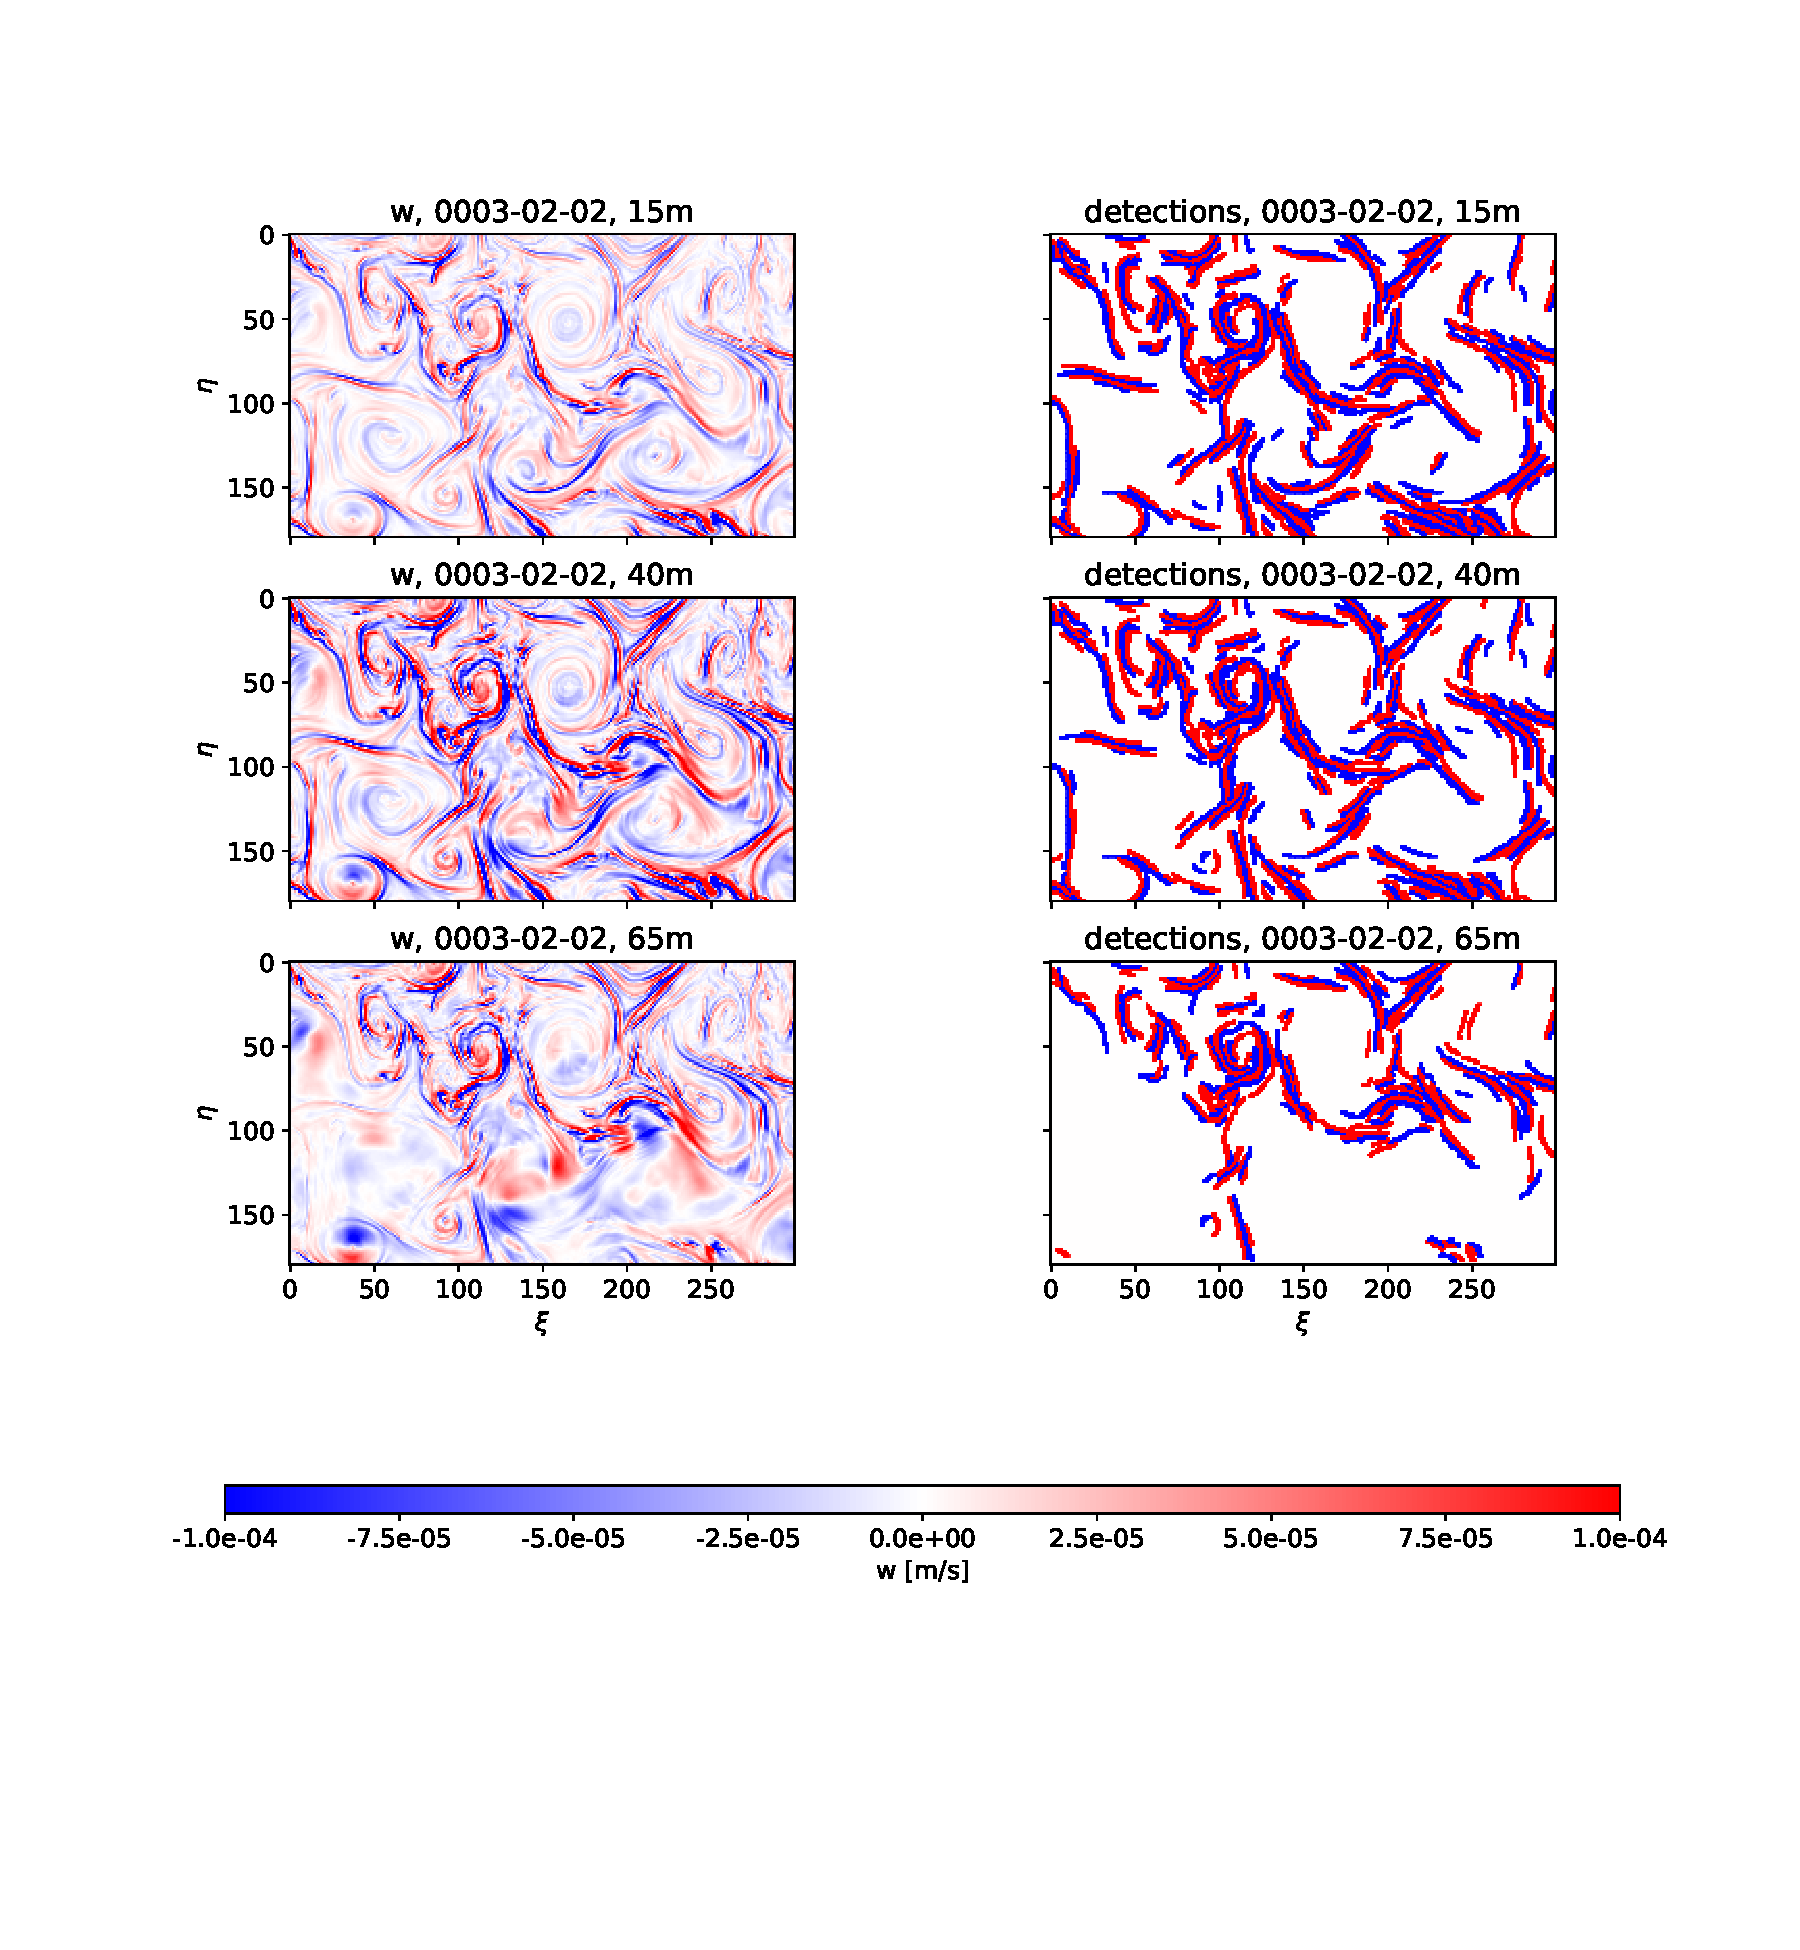
\includegraphics[width=16cm, trim=2.5cm 0 0 2cm]{figures/eval_det_subm_winter.pdf}
    \caption[Detection results for HR in winter: I]{\textbf{Detection results for HR in winter: I}. Data from 0003-02-02 is shown for different depths. The vertical velocity is shown left, the detection results right.}\label{fig:subm_det_winter}
\end{figure}

\begin{figure}
    \centering
    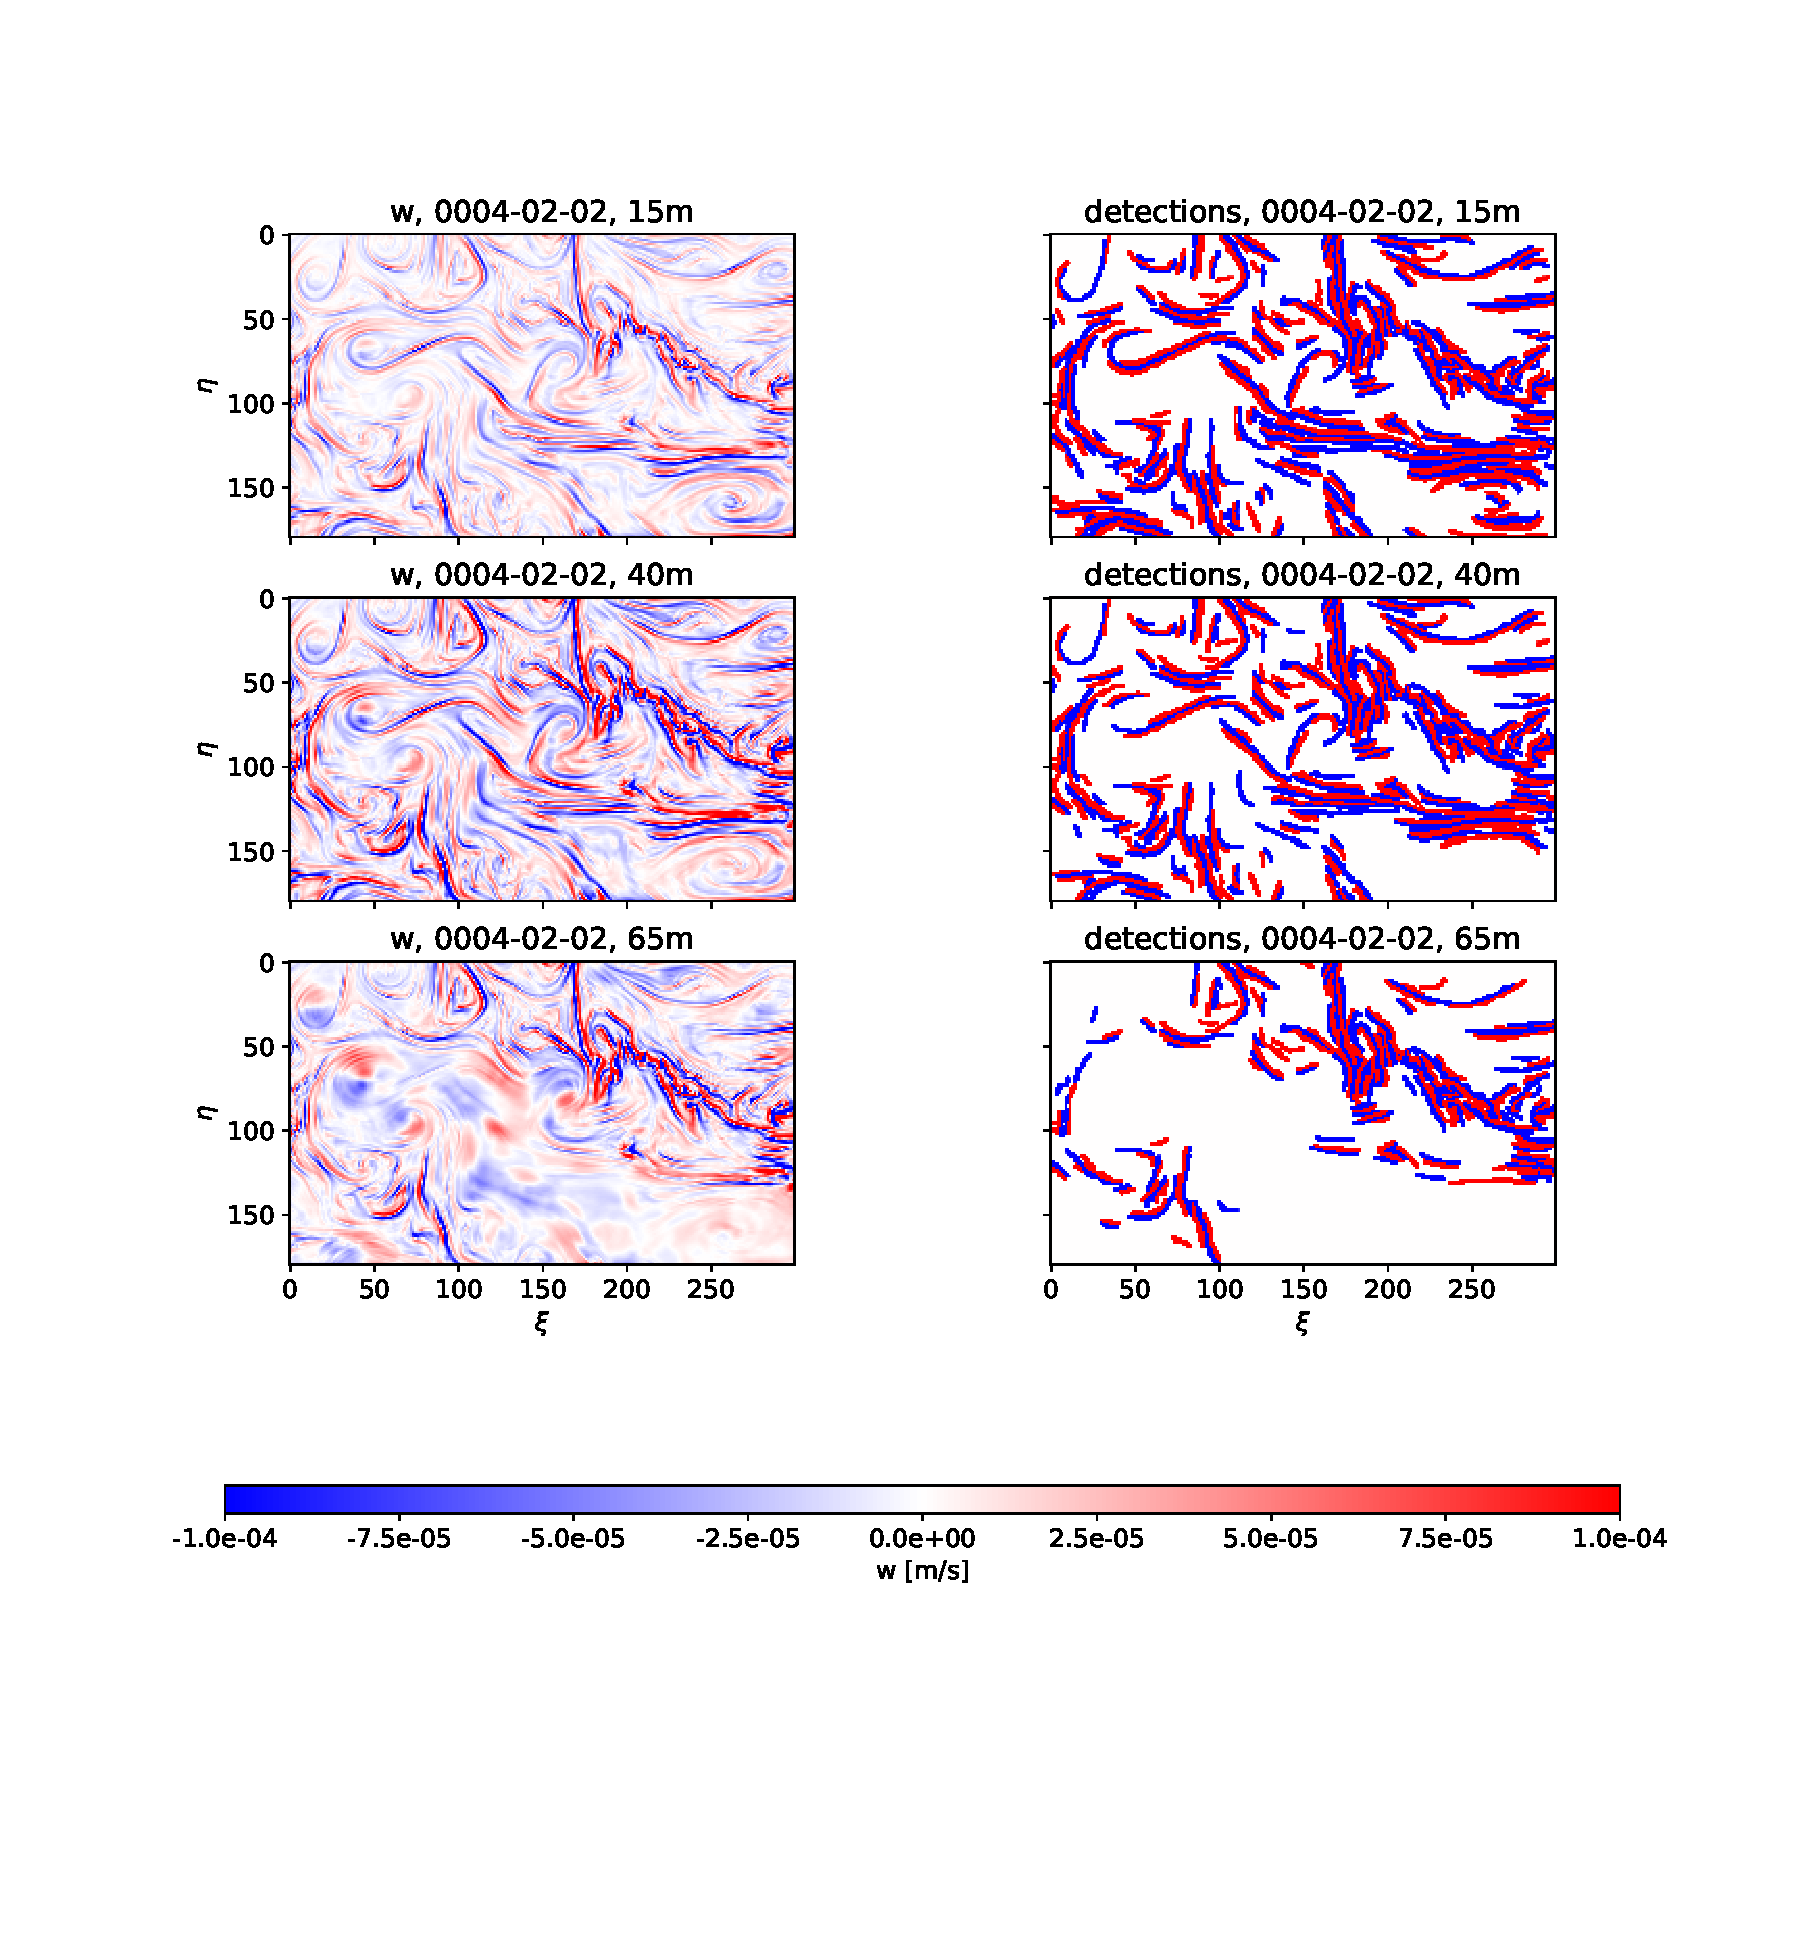
\includegraphics[width=16cm, trim=2.5cm 0 0 2cm]{figures/eval_det_subm_winter2.pdf}
    \caption[Detection results for HR in winter: II]{\textbf{Detection results for HR in winter: II}. Data from 0004-02-02 is shown for different depths. The vertical velocity is shown left, the detection results right.}\label{fig:subm_det_winter2}
\end{figure}

\begin{figure}
    \centering
    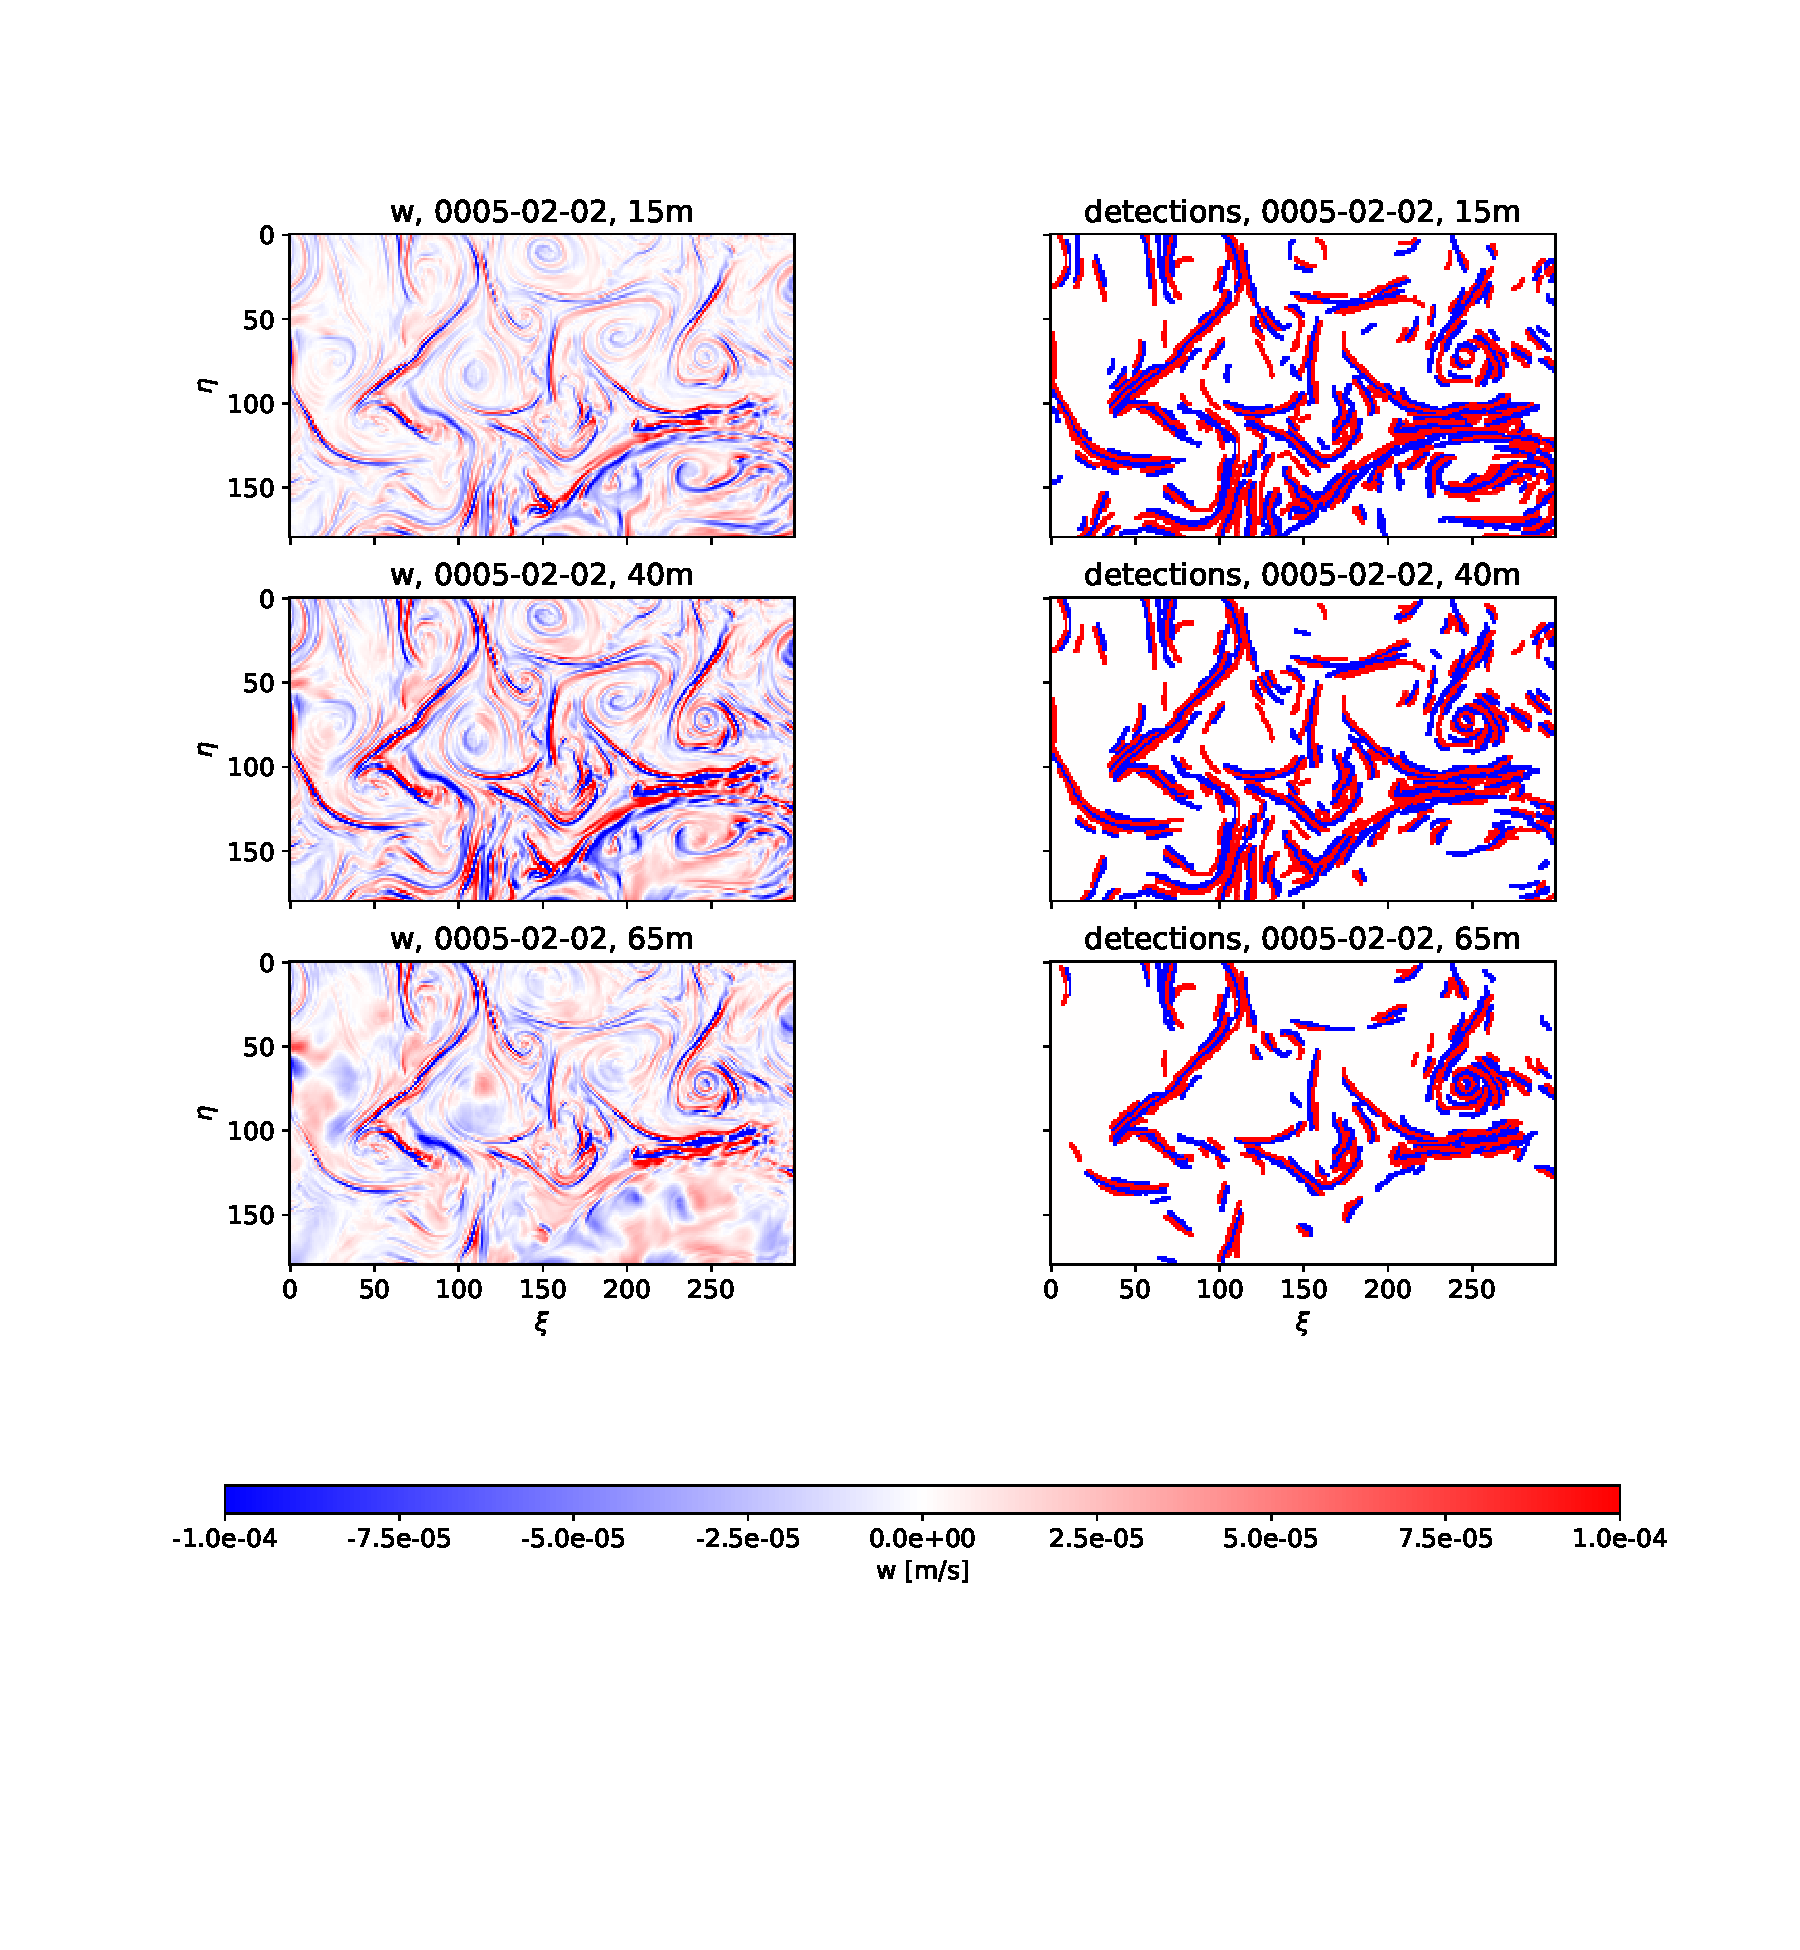
\includegraphics[width=16cm, trim=2.5cm 0 0 2cm]{figures/eval_det_subm_winter3.pdf}
    \caption[Detection results for HR in winter: III]{\textbf{Detection results for HR in winter: III}. Data from 0005-02-02 is shown for different depths. The vertical velocity is shown left, the detection results right.}\label{fig:subm_det_winter3}
\end{figure}

\begin{figure}
    \centering
    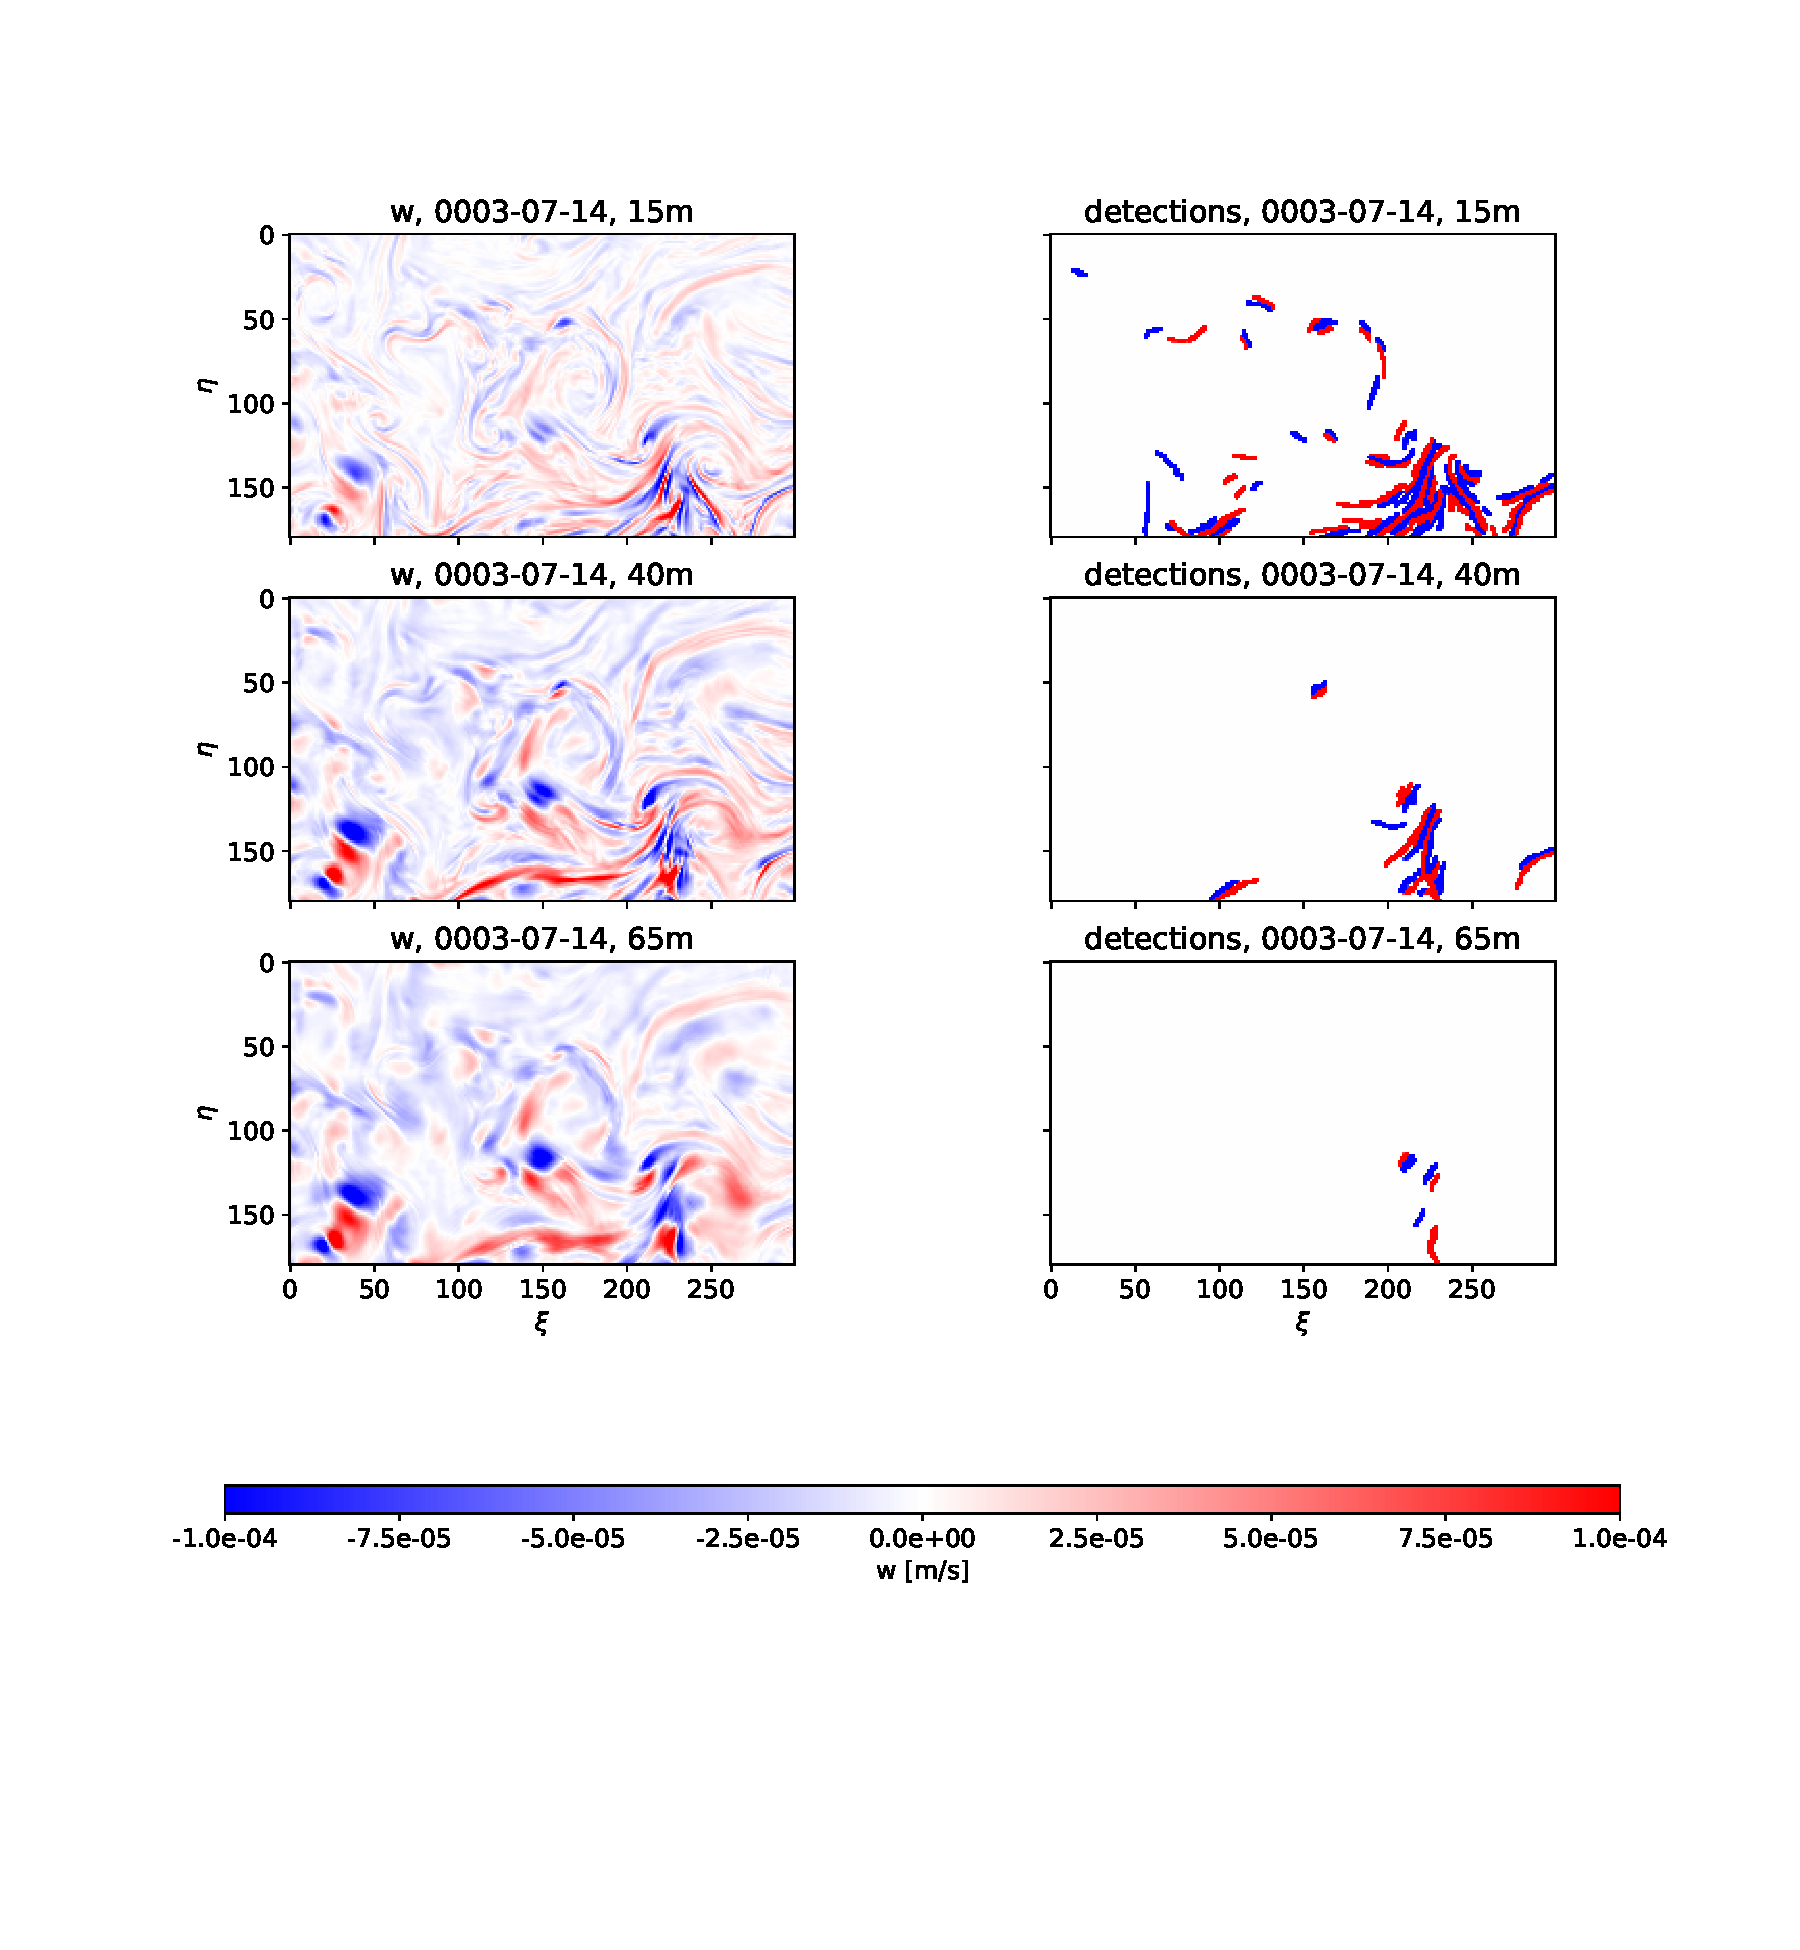
\includegraphics[width=16cm, trim=2.5cm 0 0 2cm]{figures/eval_det_subm_summer.pdf}
    \caption[Detection results for HR in summer]{\textbf{Detection results for HR in summer}. Data from 0003-07-14 is shown for different depths. The vertical velocity is shown left, the detection results right.}\label{fig:subm_det_summer}
\end{figure}

\begin{figure}
    \centering
    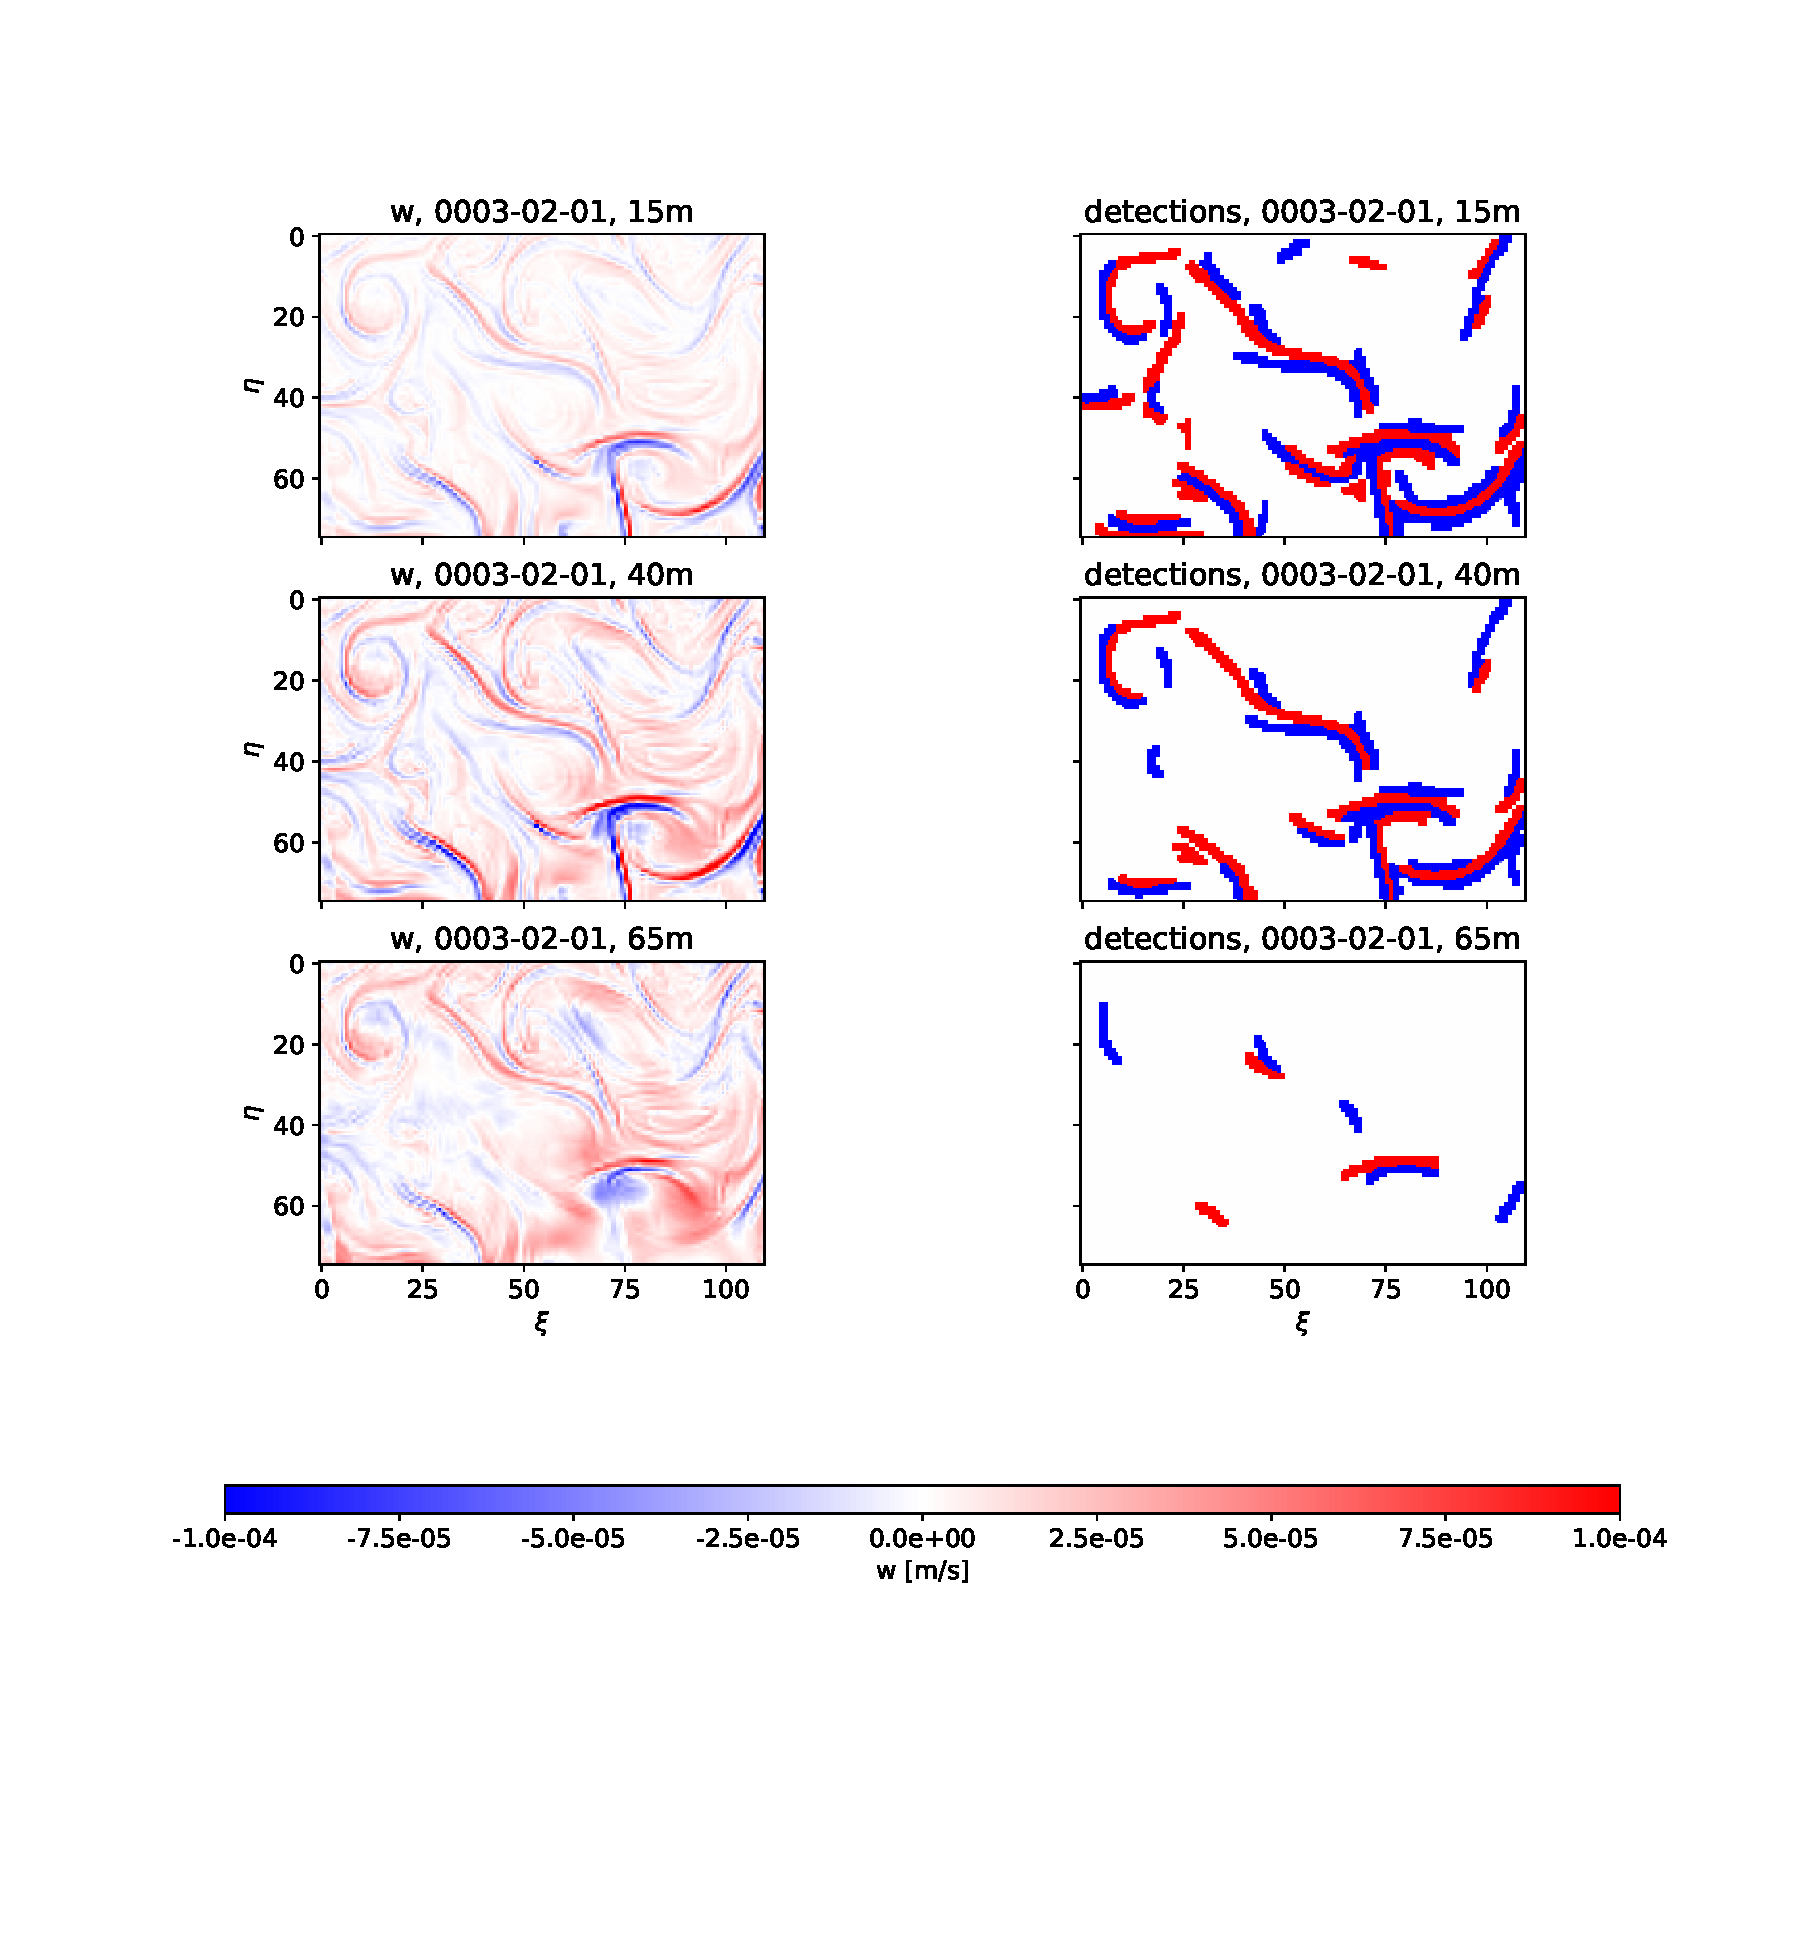
\includegraphics[width=16cm, trim=2.5cm 0 0 2cm]{figures/eval_det_meso_winter.pdf}
    \caption[Detection results for LR in winter: I]{\textbf{Detection results for LR in winter: I}. Data from 0003-02-01 is shown for different depths. The vertical velocity is shown left, the detection results right.}\label{fig:subm_det_winter_meso}
\end{figure}

\begin{figure}
    \centering
    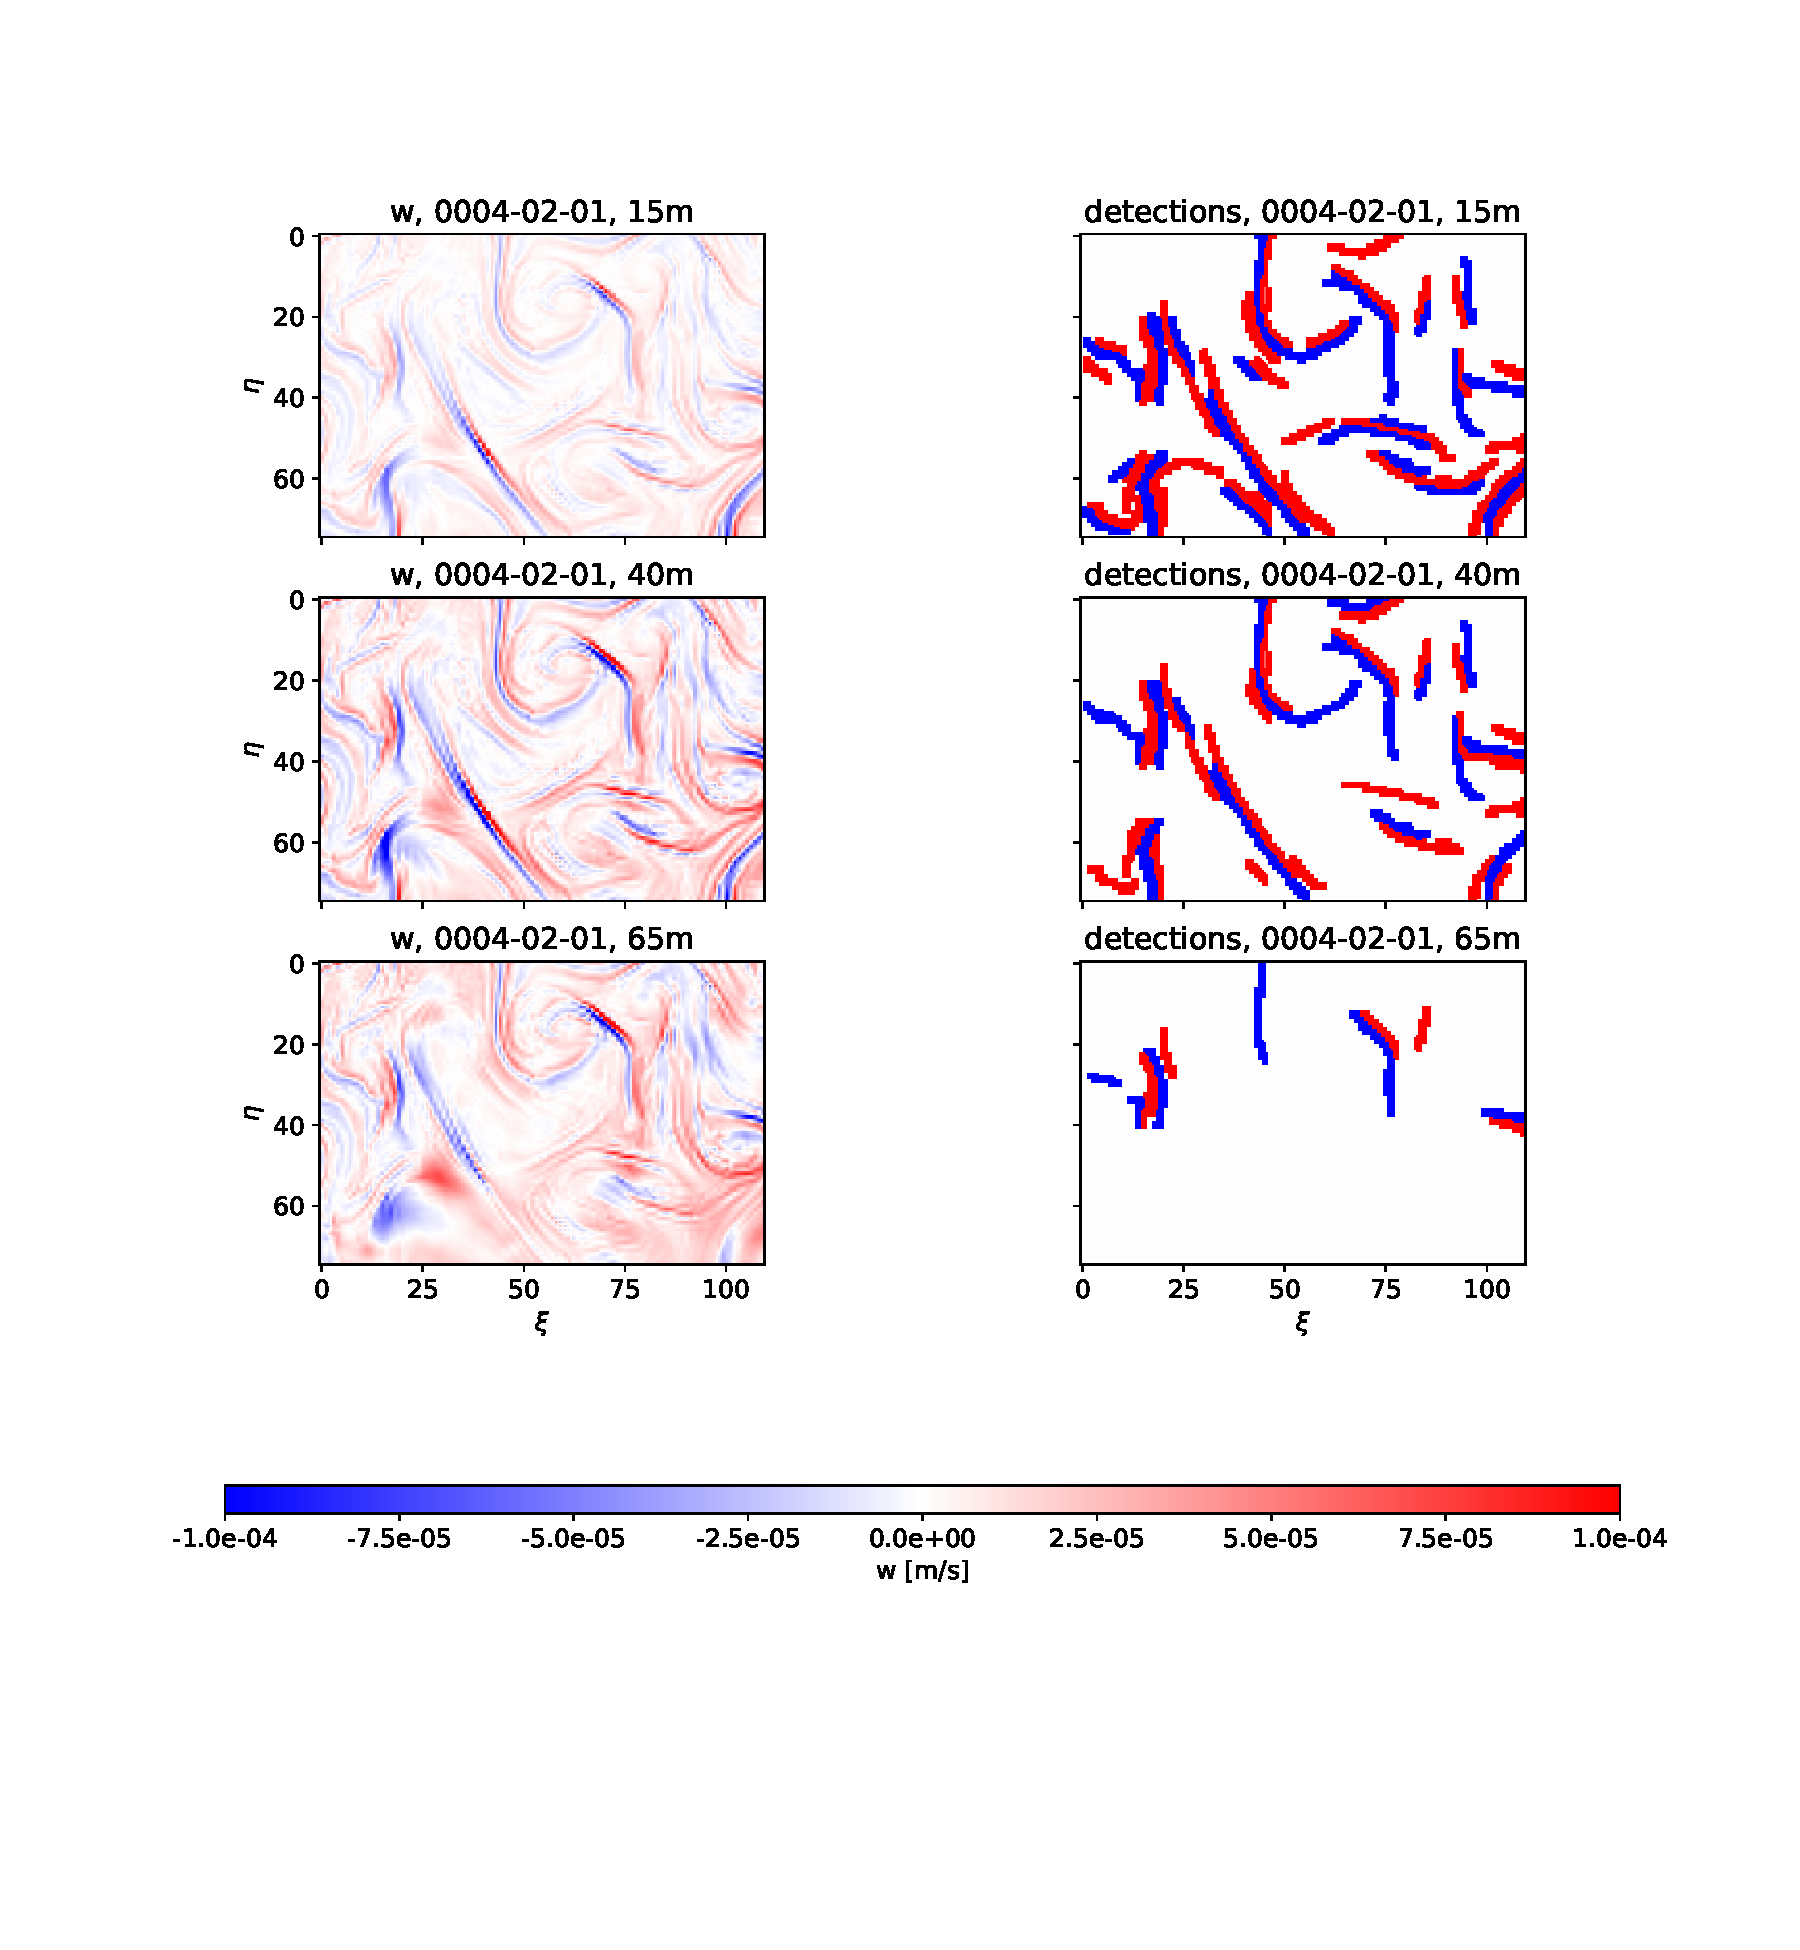
\includegraphics[width=16cm, trim=2.5cm 0 0 2cm]{figures/eval_det_meso_winter2.pdf}
    \caption[Detection results for LR in winter: II]{\textbf{Detection results for LR in winter: II}. Data from 0004-02-01 is shown for different depths. The vertical velocity is shown left, the detection results right.}\label{fig:subm_det_winter_meso2}
\end{figure}

\begin{figure}
    \centering
    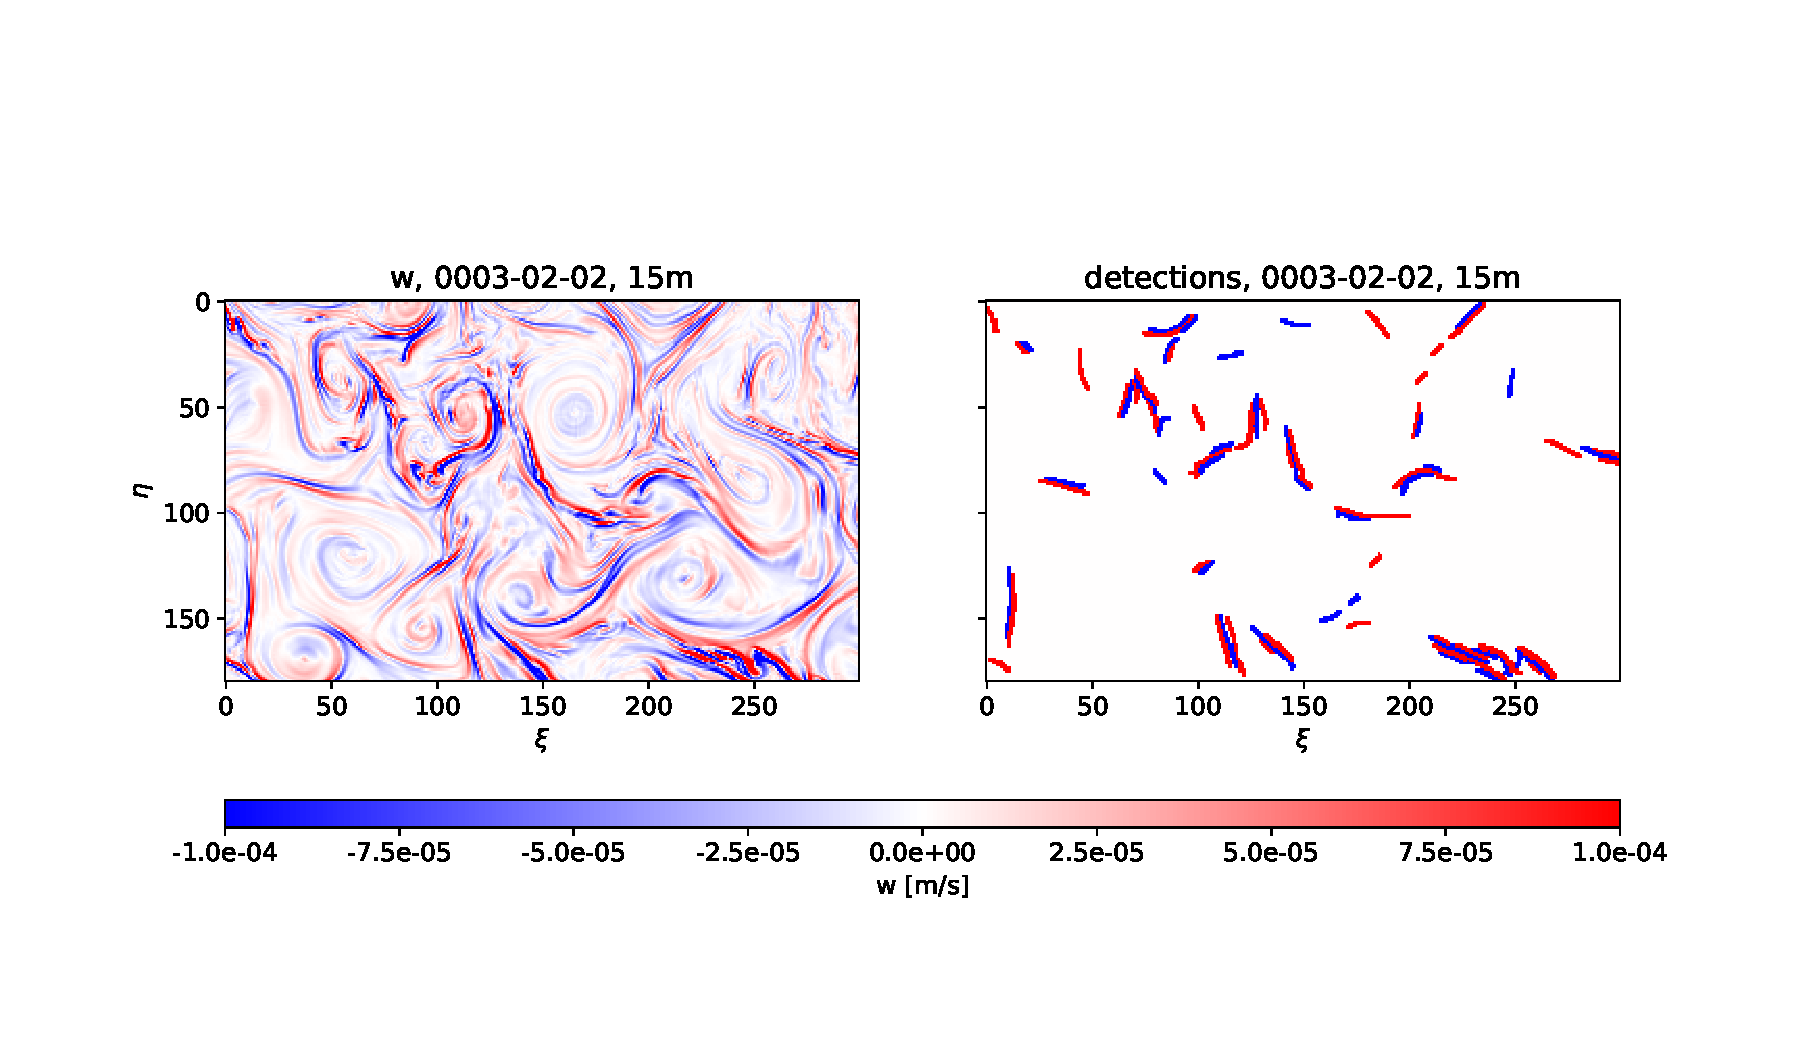
\includegraphics[width=16cm, trim=2.5cm 0 0 2cm]{figures/eval_det_sig_sm.pdf}
    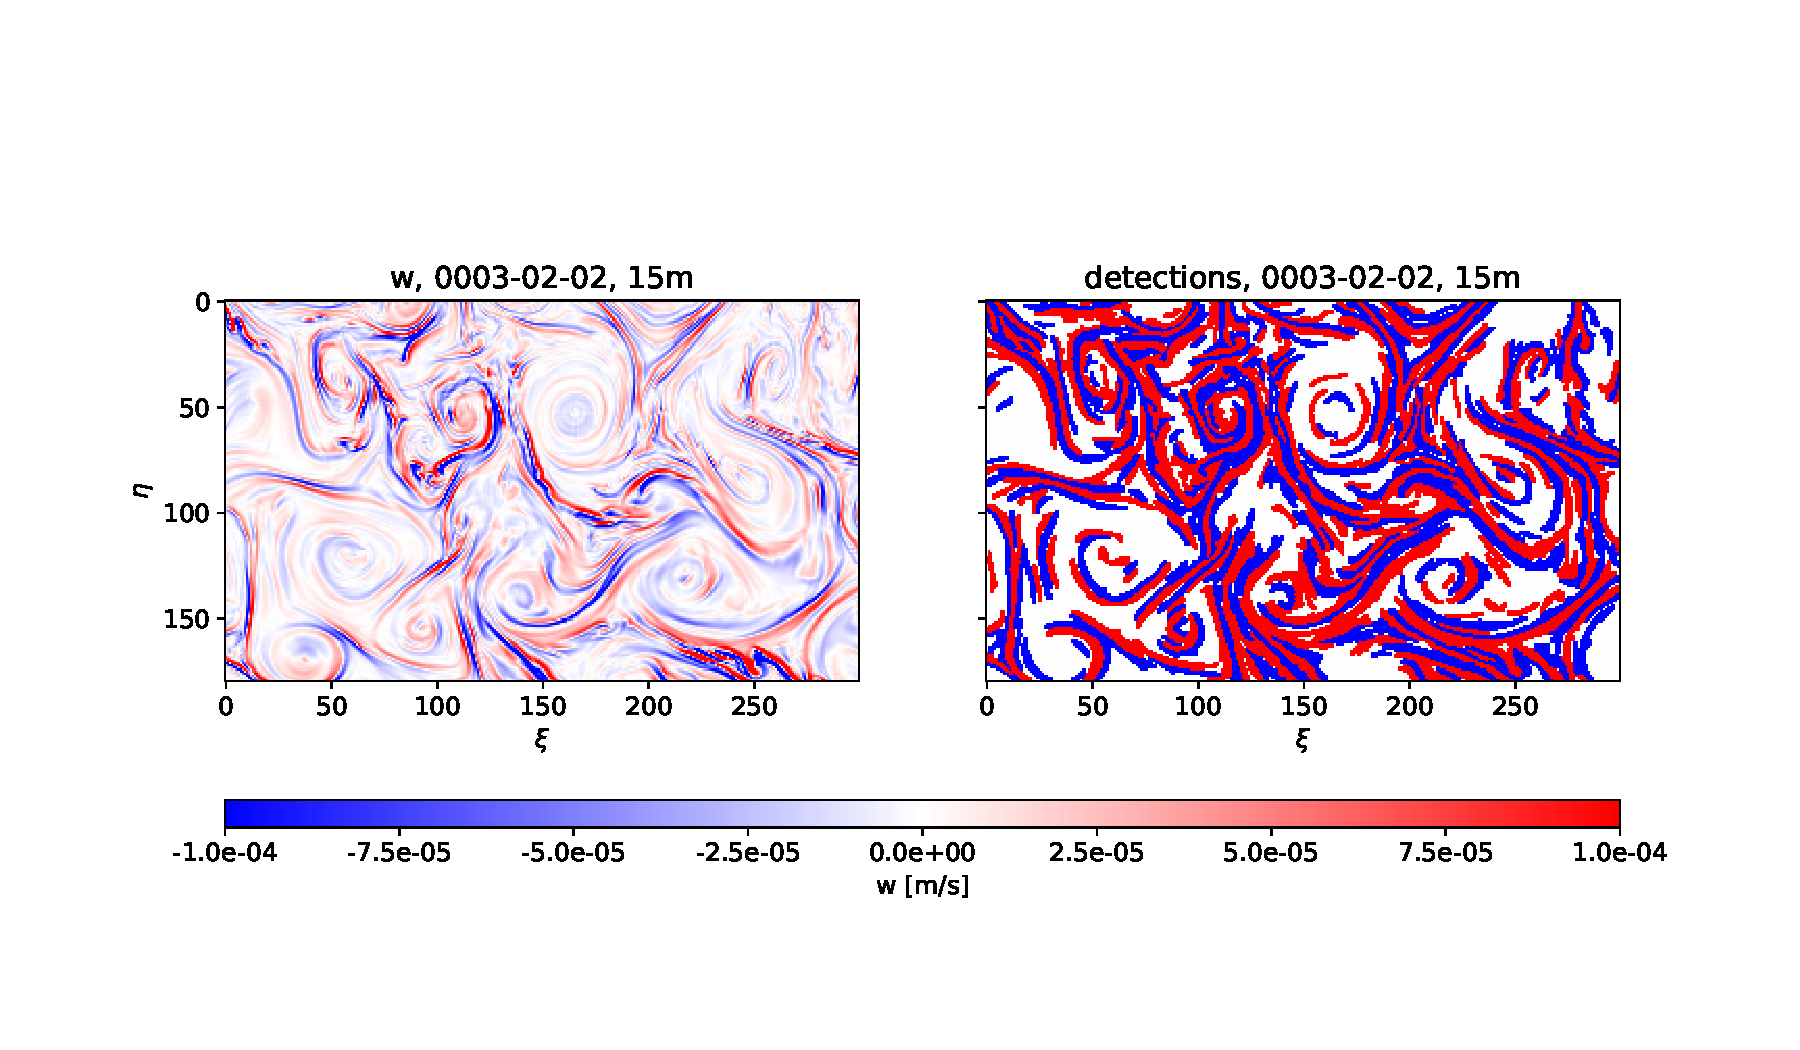
\includegraphics[width=16cm, trim=2.5cm 0 0 2cm]{figures/eval_det_sig_lg.pdf}
    \caption[Detection results for different $\sigma_\text{lat}$]{\textbf{Detection results for different $\sigma_\text{lat}$}. Data from 0003-02-01 is shown for $\sigma_\text{lat} = 1$ (top) and $\sigma_\text{lat} = 4$ (bottom). See \autoref{fig:subm_det_winter} for $\sigma_text{lat} = 2$.}\label{fig:subm_det_sigma}
\end{figure}

\begin{figure}
    \centering
    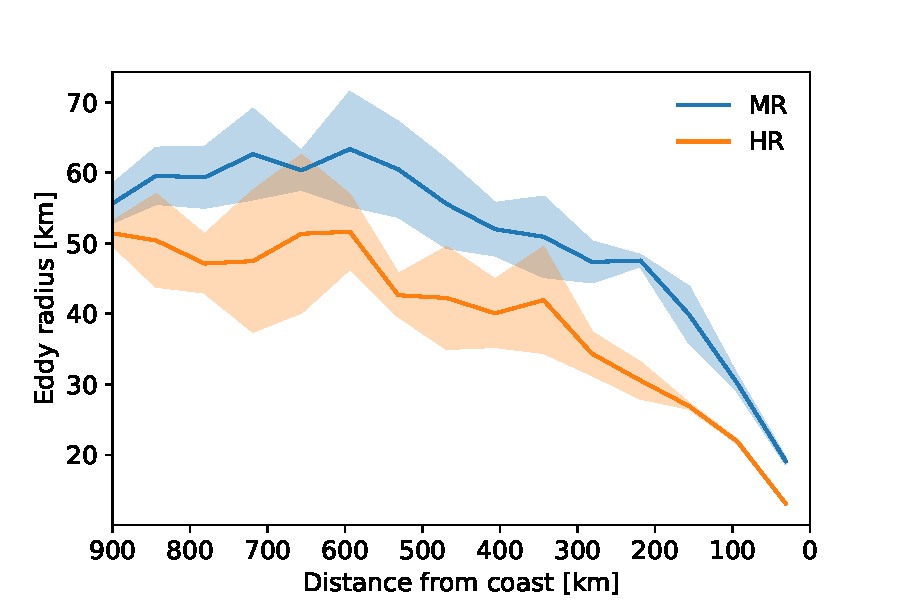
\includegraphics[width=8cm]{figures/result_eddies_d2c.pdf}
    \caption[Relative change of eddy radius with distance from coast]{\textbf{Eddy radius with distance from coast}.}
    \label{fig:meso_d2c}
\end{figure}

\begin{figure}
    \centering
    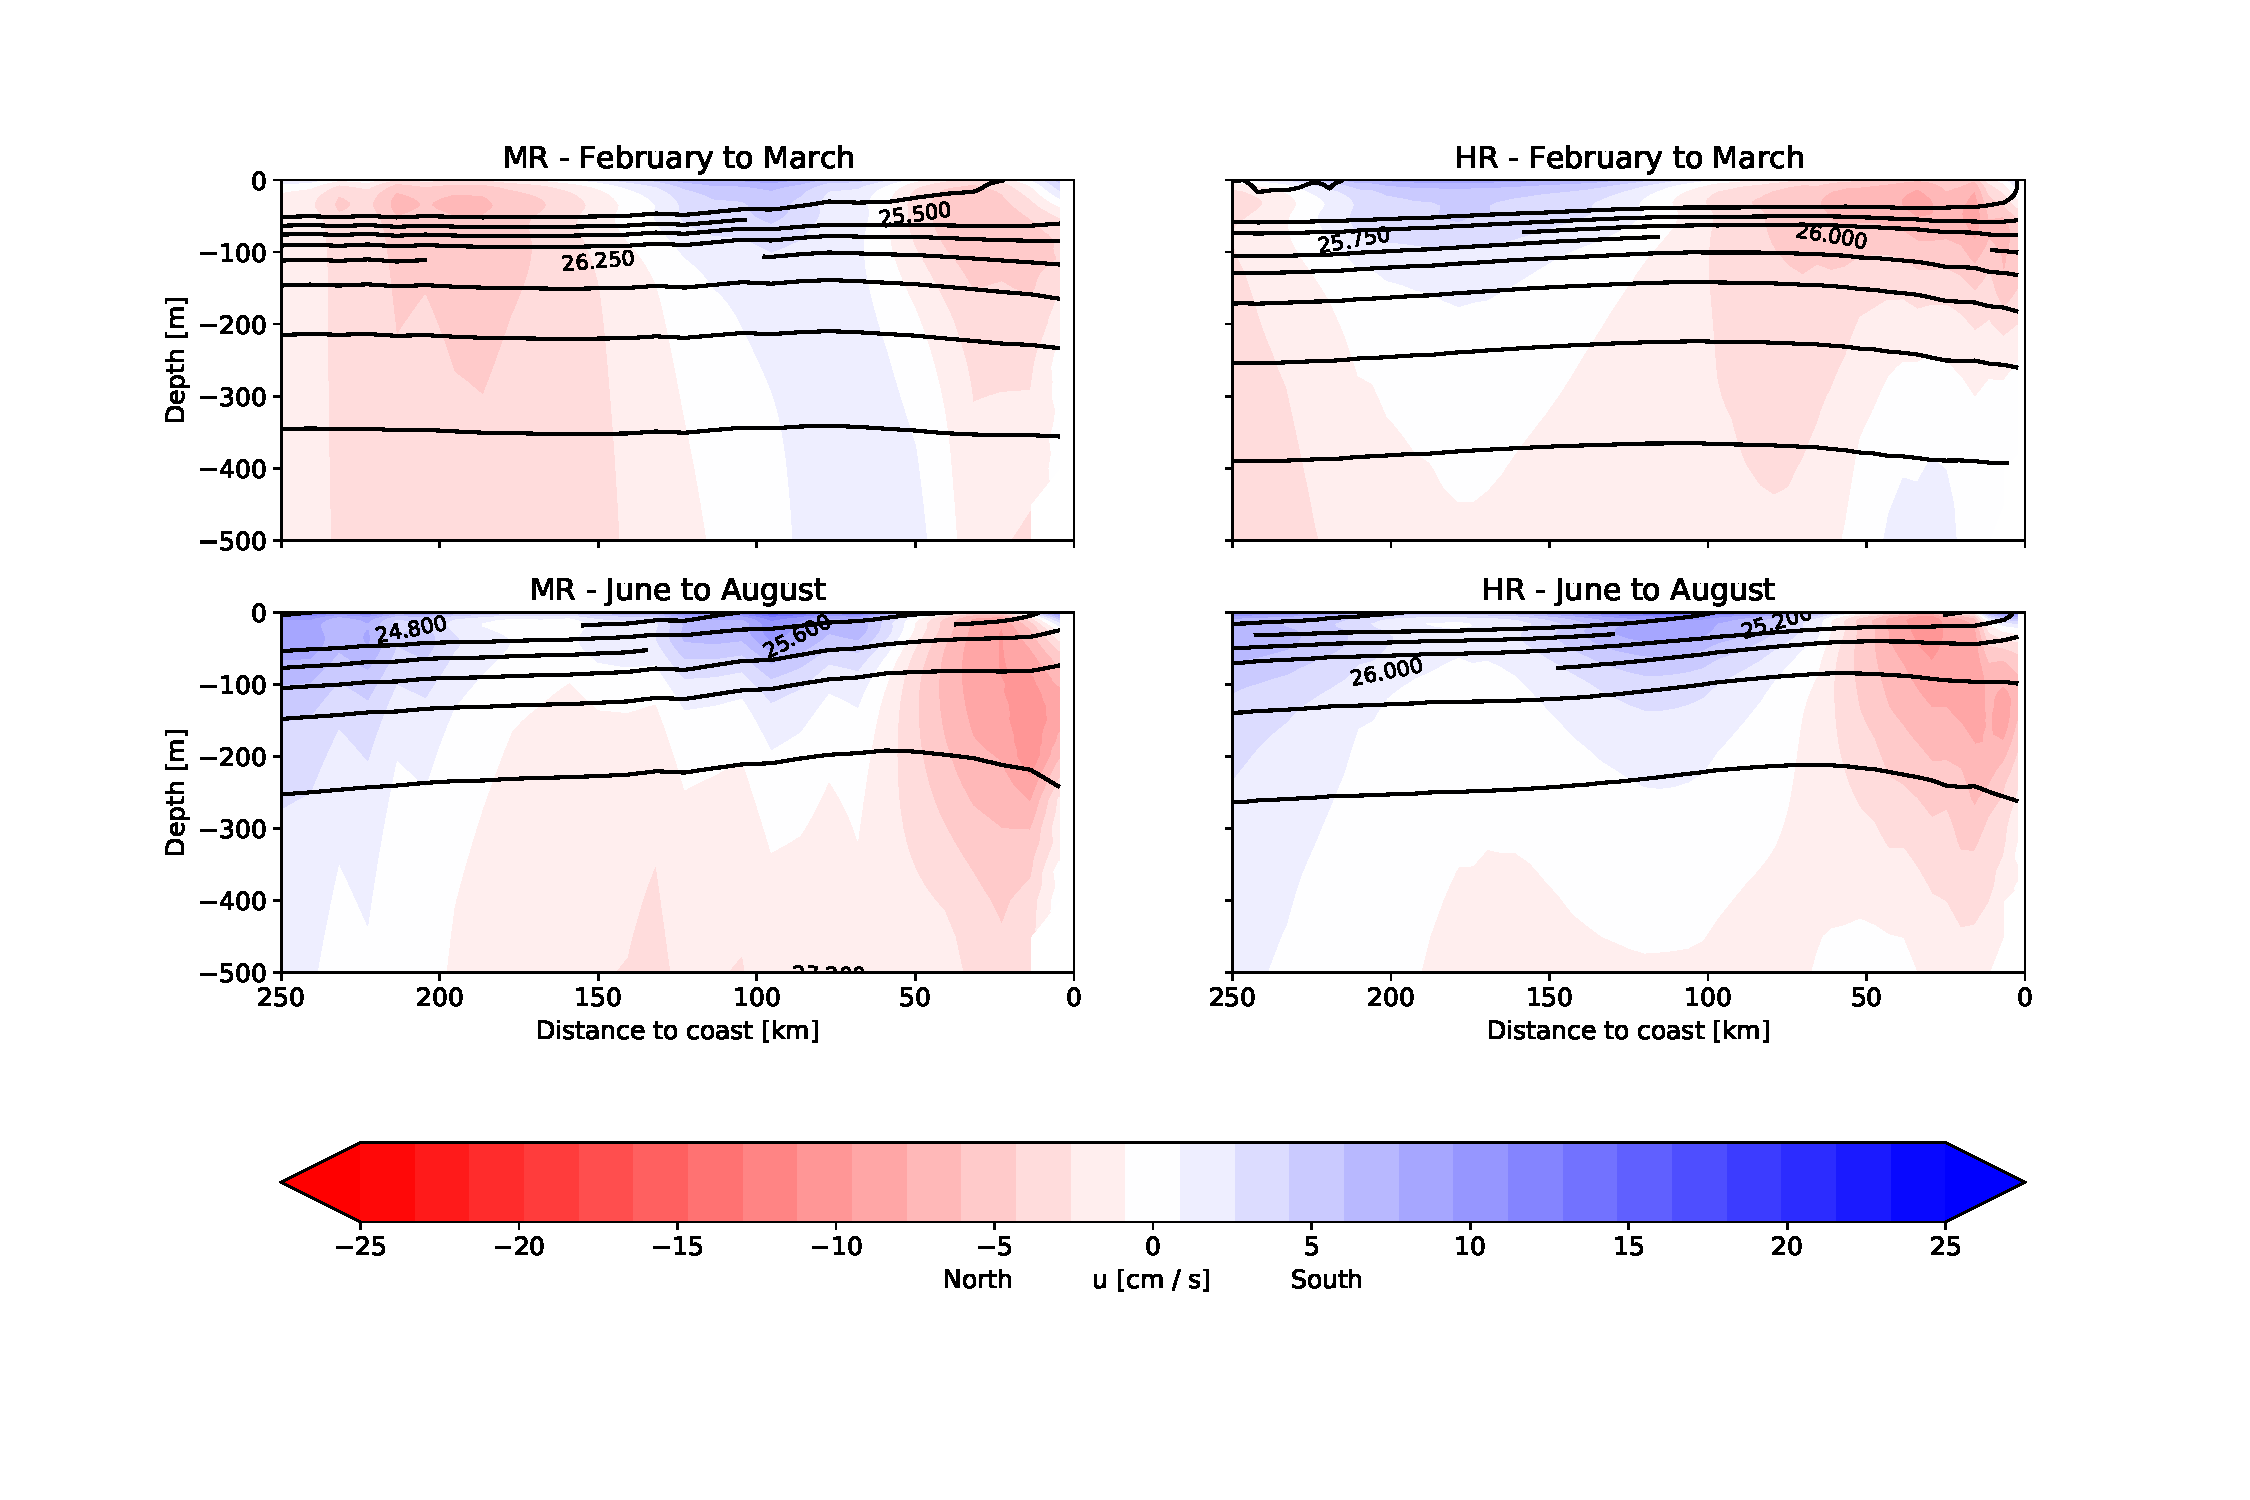
\includegraphics[width=16cm, trim=2cm 0 0 0]{figures/result_undercurrent.pdf}
    \caption[California Current and Undercurrent strength]{\textbf{California Current and Undercurrent strength}. The horizontal velocity component $u$ (parallel to coast) is shown for winter (top) and summer (bottom). The results for \ac{mr} are shown left and for \ac{hr} right. Contours represent isopycnals.}\label{fig:undercurrent}
\end{figure}

\begin{figure}
    \centering
    \hspace*{-0.2cm}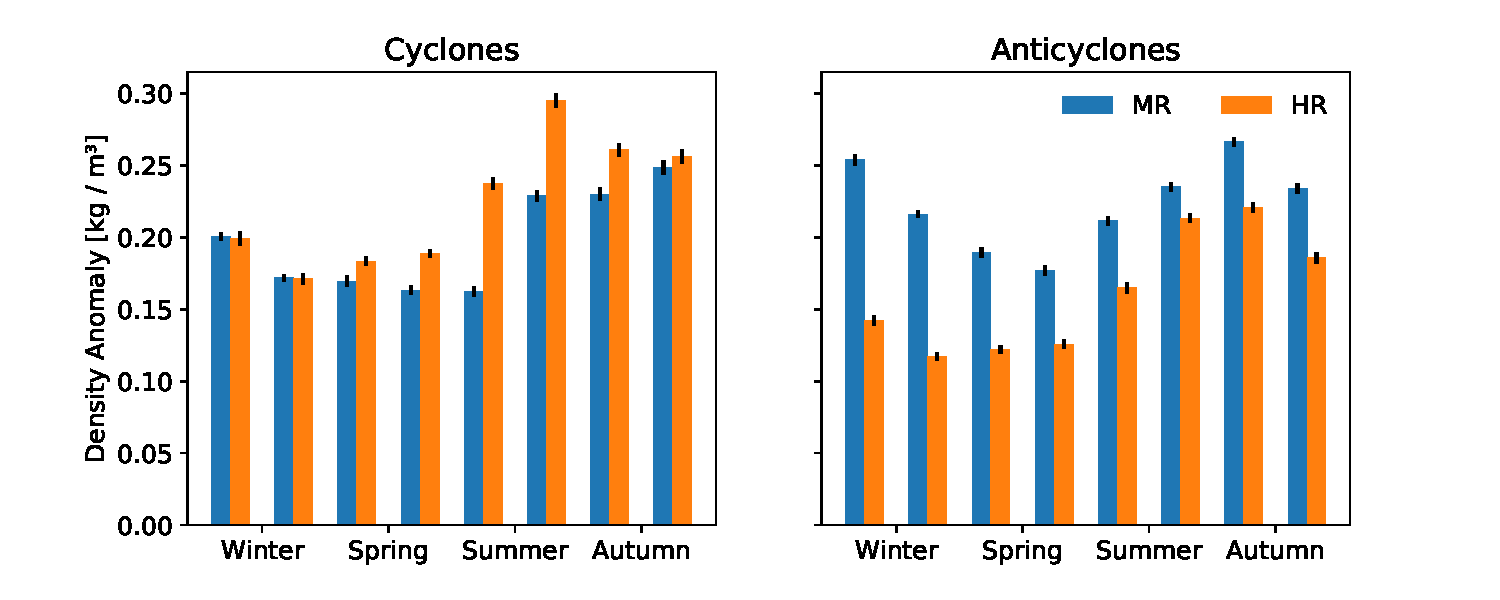
\includegraphics[width=16cm, trim=0 0 0 0]{../figures/result_eddies_density2}
    \caption[Offshore density anomaly (increased depth range)]{\textbf{Offshore density anomaly (increased depth range)}. Same as \autoref{fig:density-anomaly}, but averaged from 25m to 200m depth.}\label{fig:density-anomaly2}
\end{figure}

\begin{figure}
    \centering
    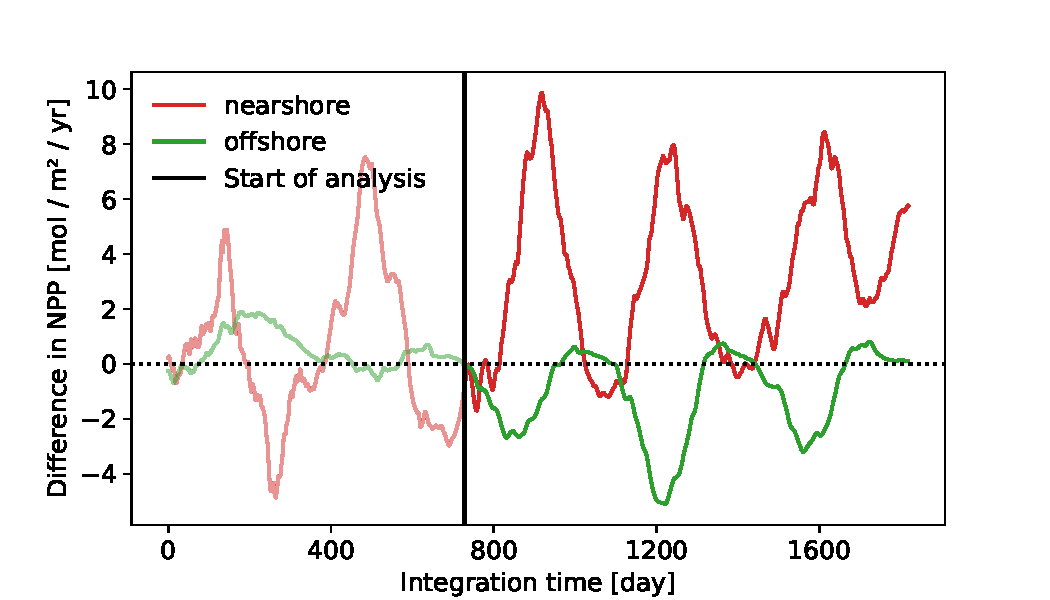
\includegraphics[width=10cm]{../figures/result_npp_drift.pdf}
    \caption[Temporal evolution of NPP difference]{\textbf{Temporal evolution of NPP difference} The difference MR - HR is shown for nearshore region (red) and offshore region (green). The curves were smoothed with a 120d rolling average. The solid black line denotes the start of analysis.}
    \label{fig:npp_drift}
\end{figure}
		\chapter{Lists}
		\listoffigures
		\listoftables
		\printbibliography
	\end{appendices}
	
	\section*{Selbstständigkeitserklärung}

\setlength{\parindent}{0em}

\vspace{3\baselineskip}
Ich versichere, dass ich diese Arbeit selbstst\"{a}ndig verfasst habe und keine
anderen als die angegebenen Quellen und Hilfsmittel benutzt habe.\par
\vspace{4\baselineskip}

Zürich, den 18.12.2020 \hspace{3cm}\dotfill

\end{document}
